\chapter{PROTOTIPAR}
El presente capítulo desarrolla la cuarta etapa del Design Thinking: Prototipar. Su propósito es construir una representación tangible de las ideas seleccionadas en el Capítulo 7, que permita visualizar las decisiones de diseño, iniciar conversaciones productivas con los usuarios y detectar errores de forma temprana (Vargas Márquez et al., 2021). Se describe la arquitectura del sistema, las reglas de interacción implementadas, el algoritmo de emparejamiento, los mecanismos de seguridad y el sistema de diseño bajo principios de IHC Afectiva del prototipo, denominado ECHOOM.

La Figura \ref{fig:flujo} presenta el flujo principal de la aplicación: la bienvenida, el registro del ánimo del día, la pantalla de Inicio, la elección de los temas de la semana, la presentación de la persona con quien se conversará, la conversación, el cierre de la semana y el Jardín.

\begin{figure}[htbp]
  \centering
  \caption{Flujo principal de ECHOOM}
  \label{fig:flujo}
  \vspace{4pt}
  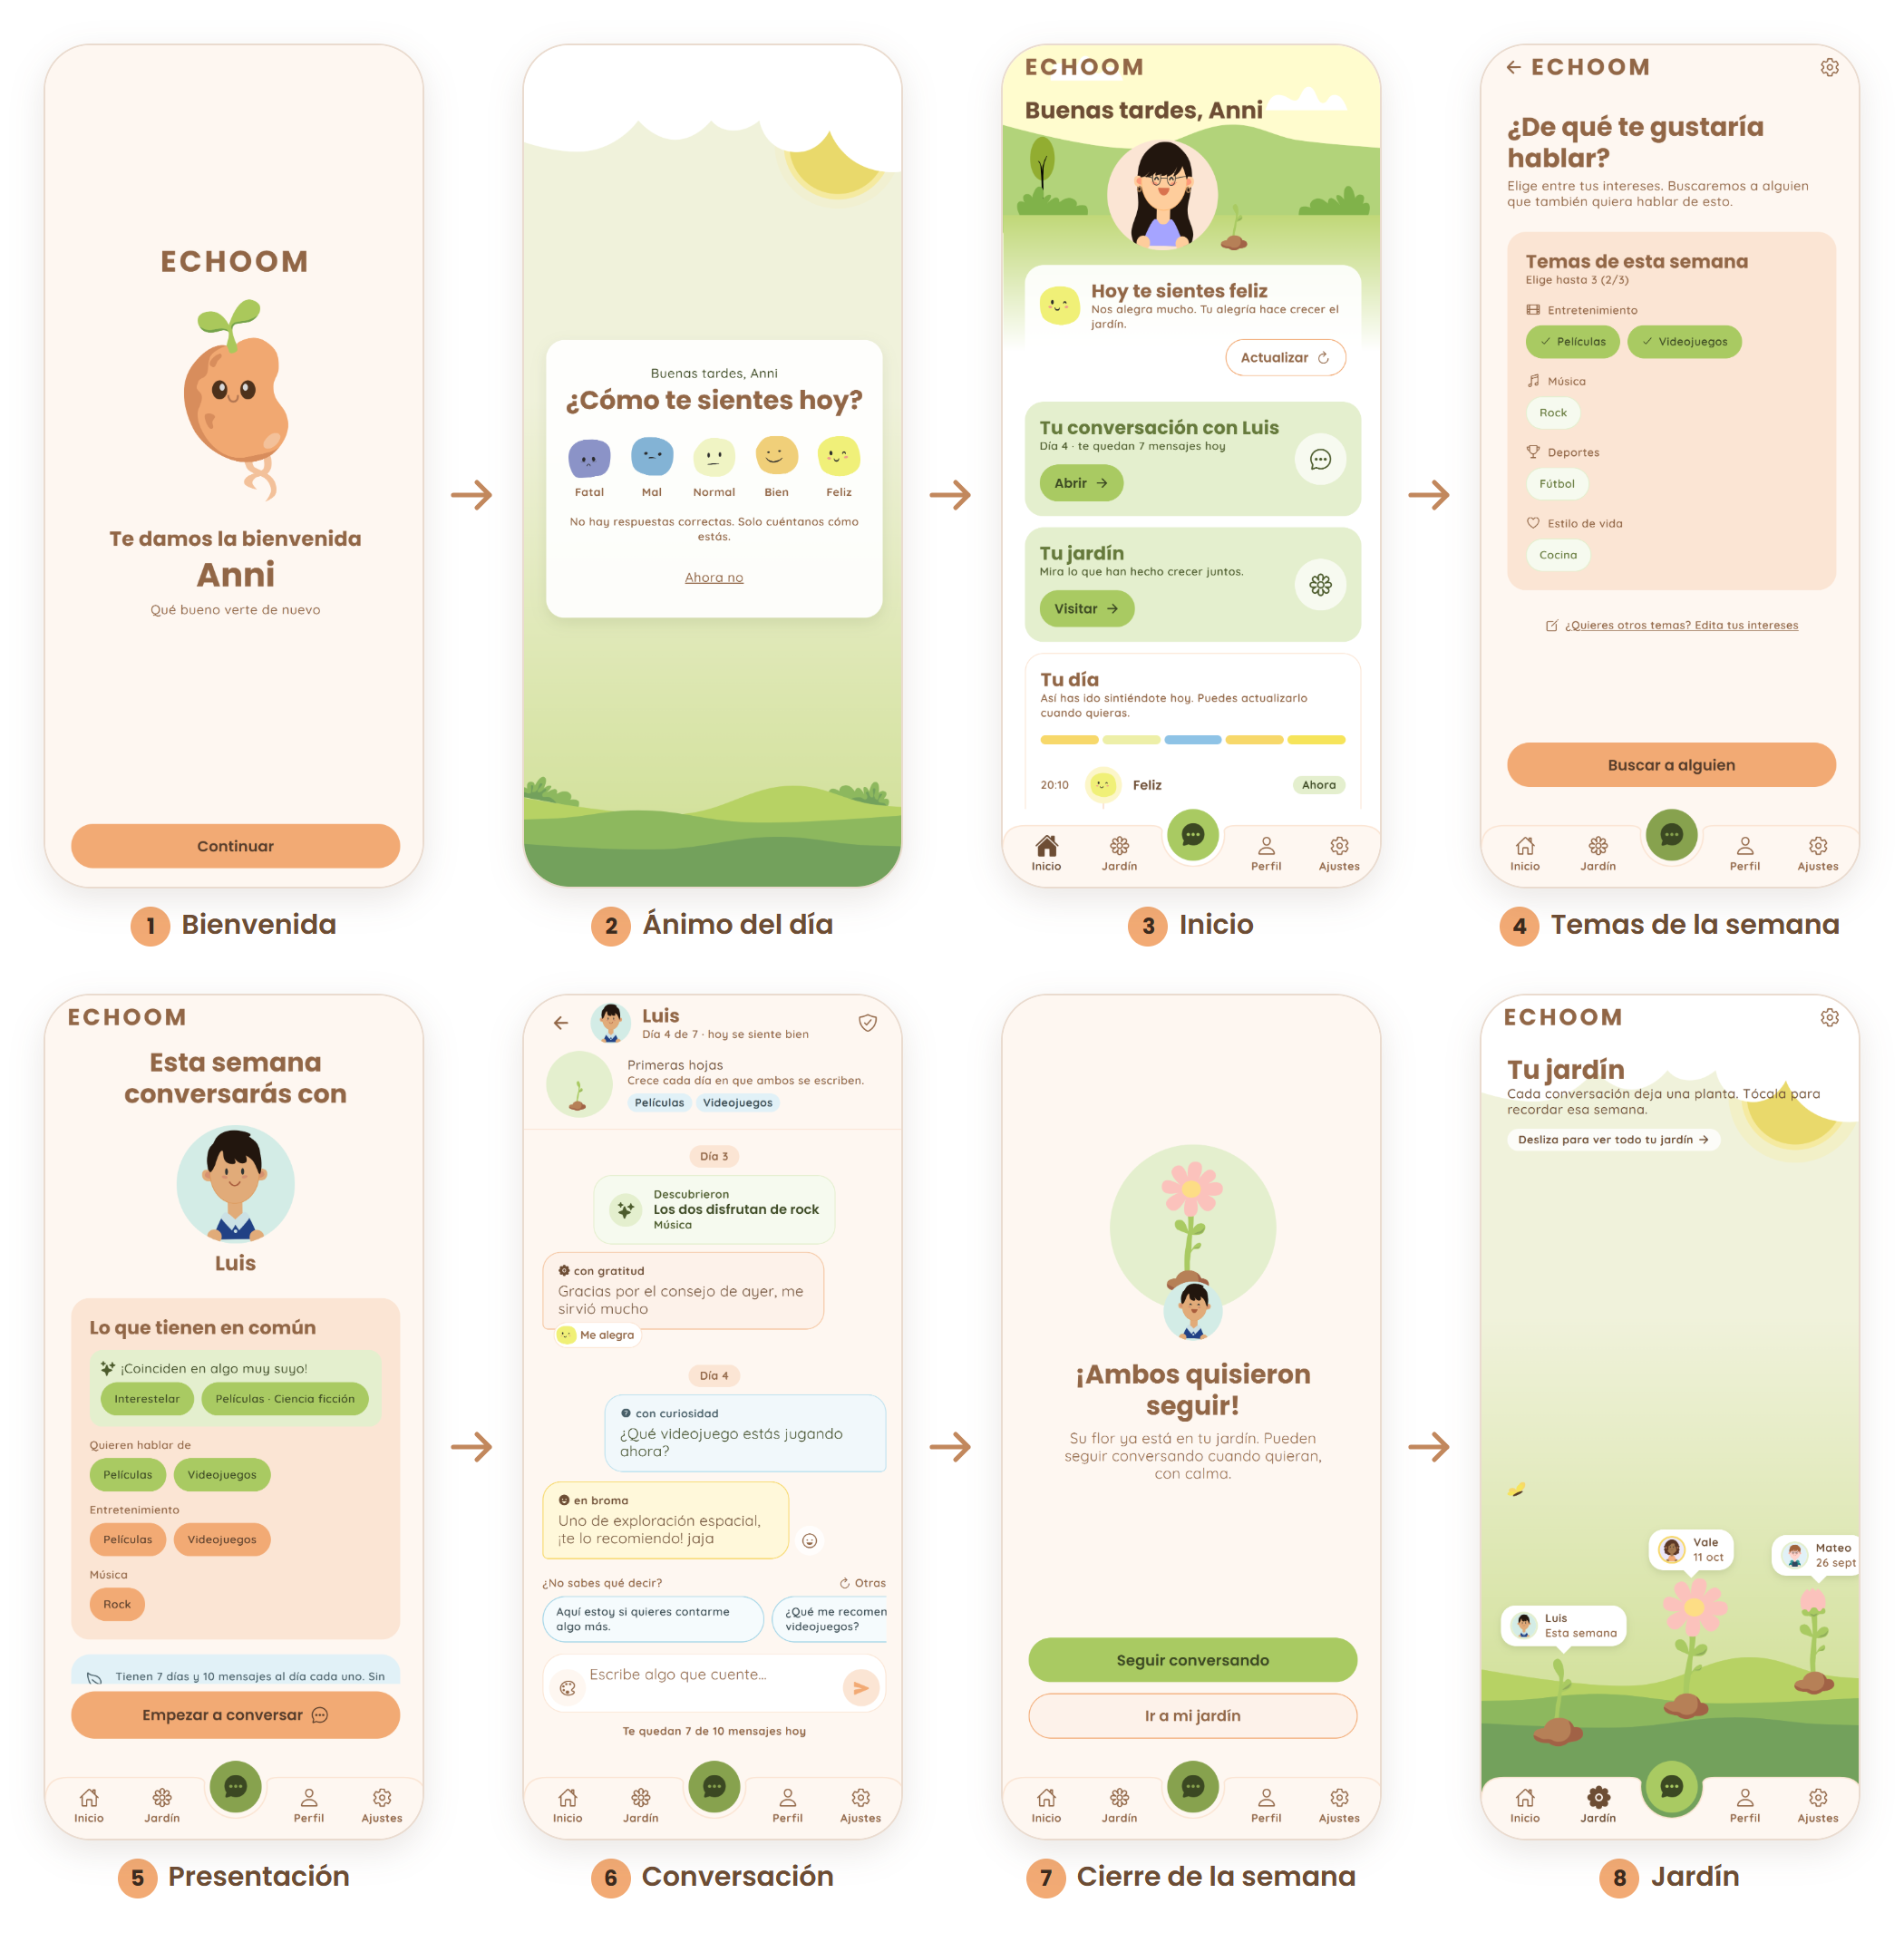
\includegraphics[width=\textwidth]{Images/methodology/prototype/flow.png}
  \vspace{4pt}
\end{figure}

\section{ARQUITECTURA}
El prototipo se desarrolló bajo una arquitectura cliente-servidor, compuesta por los elementos que se describen a continuación y se representan en la Figura \ref{fig:arquitectura}:

\begin{itemize}
    \item \textbf{Cliente:} aplicación desarrollada en React Native con Expo (TypeScript), organizada por funcionalidades: autenticación, \textit{onboarding}, inicio, conversación, jardín, perfil y ajustes. Expo permite generar el instalador de la aplicación para Android, que se utilizará en las pruebas piloto descritas en el Capítulo 9.
    \item \textbf{Servidor:} API REST desarrollada en FastAPI (Python), organizada en los módulos de autenticación, usuarios y avatar, ánimo, emparejamiento, chat, jardín, sugerencias y estado del servicio. Estos módulos comparten un núcleo común que se encarga de la seguridad (tokens JWT y contraseñas cifradas), la moderación de cada mensaje antes de guardarlo, el límite de peticiones y los mensajes de error en español.
    \item \textbf{Base de datos:} PostgreSQL, con migraciones versionadas mediante Alembic. Se optó por un modelo relacional en lugar de uno documental, dado que los datos del sistema (usuarios, conversaciones, mensajes y decisiones) presentan relaciones estructuradas entre sí, y porque PostgreSQL permite bloquear el proceso de emparejamiento para evitar que dos búsquedas simultáneas generen parejas duplicadas.
    \item \textbf{Servicio externo:} Google Knowledge Graph Search API, consultada únicamente desde el servidor para proteger la clave de acceso, utilizada para el autocompletado de gustos específicos (Google, s.f.; sección 8.4).
    \item \textbf{Servicio de correo:} API de Brevo, utilizada para enviar los códigos que confirman el correo y permiten recuperar la contraseña. Durante el desarrollo, los correos se capturan localmente con Mailpit.
\end{itemize}

\begin{figure}[htbp]
  \centering
  \caption{Arquitectura cliente-servidor de ECHOOM}
  \label{fig:arquitectura}
  \vspace{4pt}
  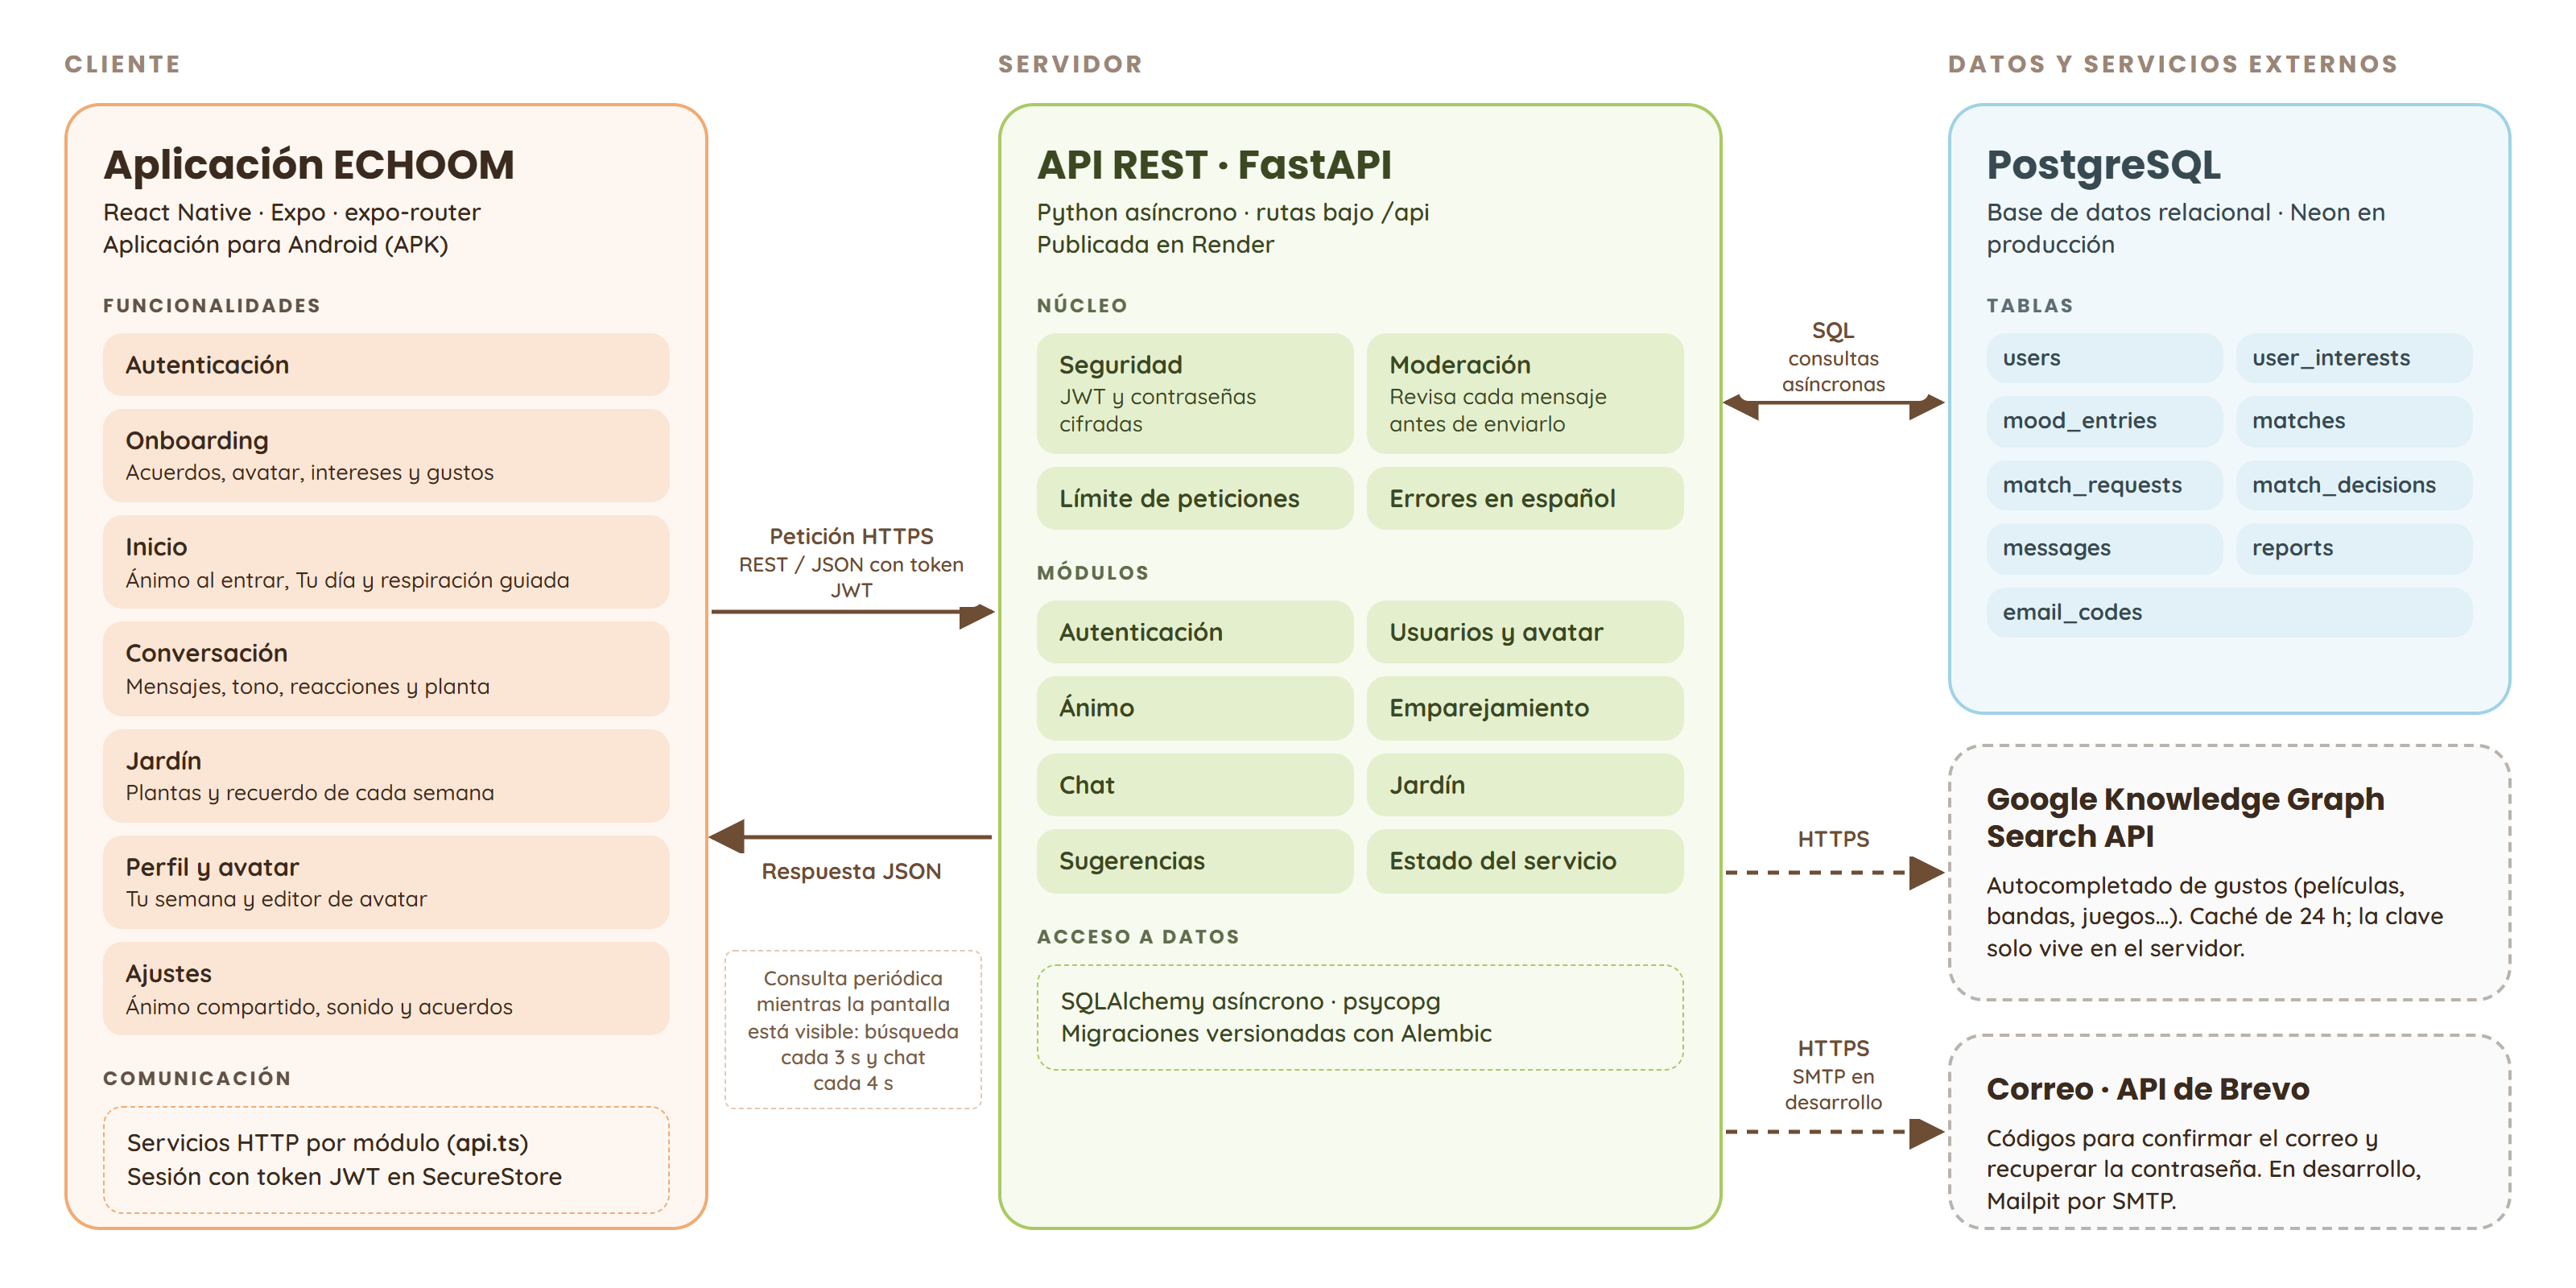
\includegraphics[width=\textwidth]{Images/methodology/prototype/architecture.png}
  \vspace{4pt}
\end{figure}

La aplicación consulta periódicamente al servidor para recibir mensajes nuevos y para verificar si ya se formó una pareja (cada 4 segundos dentro de una conversación activa, y cada 3 a 5 segundos durante la búsqueda), y únicamente mientras la pantalla correspondiente está visible, con el fin de equilibrar la capacidad de respuesta percibida con el consumo de recursos del dispositivo.

En cuanto a la calidad del software, el servidor cuenta con 80 pruebas automatizadas que verifican los módulos de autenticación (incluida la confirmación del correo con código), perfil, emparejamiento, chat, reglas semanales, jardín, reportes, sugerencias y moderación de mensajes. Adicionalmente, el flujo completo de la aplicación fue probado de principio a fin con dos usuarios simulados.

\subsection{Despliegue para la prueba piloto}
Para que los participantes puedan usar el prototipo desde sus propios dispositivos, el sistema se publicó en servicios con planes gratuitos que no requieren tarjeta de crédito:

\begin{itemize}
    \item La API se publica en Render, que vuelve a desplegarla automáticamente con cada cambio registrado en el repositorio de GitHub.
    \item La base de datos se aloja en Neon, un servicio administrado de PostgreSQL.
    \item Los correos con códigos de verificación se envían mediante la API de Brevo, dado que el plan gratuito de Render bloquea el envío por SMTP.
    \item La aplicación se instala en los teléfonos Android de los participantes como un archivo APK generado con EAS Build de Expo.
\end{itemize}

Como limitación, el servidor gratuito se suspende tras 15 minutos sin uso, y la primera petición posterior tarda entre 30 y 50 segundos en responder; por ello, antes de cada sesión de prueba conviene abrir la aplicación para reactivarlo.

\section{REGLAS DE LA INTERACCIÓN}
La Tabla \ref{tab:reglas_interaccion} resume los parámetros que rigen la interacción dentro del prototipo. Estos valores constituyen hipótesis de diseño derivadas de la literatura y de la evidencia primaria recolectada en los Capítulos 5 y 6, y se someterán a validación durante la prueba piloto (Capítulo 9).

\begin{longtable}{
  >{\raggedright\arraybackslash}p{0.38\textwidth}
  >{\raggedright\arraybackslash}p{0.52\textwidth}
}
\caption{Reglas de la interacción}\label{tab:reglas_interaccion}\\
\toprule
\textbf{Regla} & \textbf{Valor} \\
\midrule
\endfirsthead
\multicolumn{2}{l}{\textit{Tabla \thetable{} (continuación)}} \\[4pt]
\toprule
\textbf{Regla} & \textbf{Valor} \\
\midrule
\endhead
\midrule
\multicolumn{2}{r}{\textit{Continúa en la siguiente página}} \\
\endfoot
\bottomrule
\endlastfoot

Duración de una conversación & 7 días \\
Días de gracia para decidir & 3 (del día 7 al 10) \\
Mensajes por persona y por día & 10 \\
Largo máximo de un mensaje & 500 caracteres \\
Tonos de mensaje & 6, opcionales \\
Reacciones & 5 caras de ánimo, una por mensaje recibido; no cuentan como mensaje \\
Etapas de la planta & 7, una por día de la semana: semilla, brote, tallito, primeras hojas, capullo, capullo creciendo y flor completa. Avanza una etapa por cada día en que ambos usuarios escriben; si ambos deciden continuar, queda en flor \\
Ánimo visible para la pareja & Solo el de las últimas 24 horas; puede desactivarse \\
Duración máxima de una búsqueda & Hasta 24 horas; el usuario puede salir y la búsqueda continúa en segundo plano \\
Temas por búsqueda & Hasta 3, seleccionados entre los propios intereses del usuario \\
Intereses mínimos requeridos & 3 \\

\end{longtable}

\noindent\textit{Nota.} Elaboración propia.

El límite diario de mensajes busca que cada mensaje sea redactado y dirigido personalmente a la otra persona, el tipo de comunicación que Burke y Kraut (2016) asociaron con mejoras en el bienestar, y evita a la vez incorporar elementos orientados a prolongar el tiempo de uso (Montag et al., 2019), en coherencia con la asociación entre el uso problemático de las redes sociales y una mayor soledad (Feng et al., 2026). Diez mensajes diarios permiten sostener una conversación fluida, incluso con respuestas breves como una risa, sin perder el carácter de micro-interacción que invita a cuidar cada mensaje; además, las reacciones permiten responder sin consumir uno. Este valor constituye una hipótesis de diseño que se validará en la prueba piloto (Capítulo 9).

\section{ALGORITMO DE EMPAREJAMIENTO}
Cuando un usuario inicia una búsqueda, el sistema lo compara con las personas que se encuentran buscando pareja en ese mismo momento. Solo se consideran aquellas que comparten al menos uno de los temas elegidos para la búsqueda, y entre ellas se selecciona a la que obtiene el puntaje de afinidad más alto, calculado mediante la siguiente fórmula:

\begin{quote}
\textbf{Puntaje = 3 × temas en común + 1 × intereses en común + 2 × subtemas en común + 4 × ejemplos en común}
\end{quote}

Esta fórmula otorga mayor peso a los niveles más específicos de afinidad: compartir un ejemplo concreto (por ejemplo, la misma película) pesa más que compartir únicamente la categoría general (por ejemplo, ``Películas''). Este diseño responde directamente a los hallazgos de los Capítulos 5 y 6, según los cuales los usuarios valoran la posibilidad de conectar a partir de gustos específicos y particulares, y es coherente con el meta-análisis de Montoya et al. (2008), según el cual la similitud real entre las personas se asocia con la atracción interpersonal, especialmente en interacciones breves o iniciales.

La comparación de textos ignora mayúsculas, espacios y tildes (por ejemplo, ``Iron Man 2'' equivale a ``iron man 2''). El sistema garantiza que nunca se repita una pareja ya formada previamente, y un bloqueo a nivel de base de datos evita que dos búsquedas simultáneas generen parejas duplicadas.

Lo que ambos usuarios comparten no se muestra solo al inicio. Dentro de la conversación, bajo la planta, se ven los temas en común, y cada día, junto al separador del día, se revela una coincidencia más (por ejemplo, ``Hoy descubrieron: a los dos les gusta \textit{Interestelar}''), ordenadas de la más específica a la más general. La similitud percibida acerca a las personas (Byrne, 1971), y compartir gustos poco comunes genera más atracción que compartir los populares (Alves, 2018); por ello se revela primero la película concreta y después el género. Revelar las coincidencias de forma progresiva, una por día, ofrece un motivo nuevo para conversar y se asemeja a la apertura gradual que genera cercanía entre desconocidos (Aron et al., 1997).

La Figura \ref{fig:emparejamiento} resume los pasos del algoritmo de emparejamiento.

\begin{figure}[htbp]
  \centering
  \caption{Algoritmo de emparejamiento}
  \label{fig:emparejamiento}
  \vspace{4pt}
  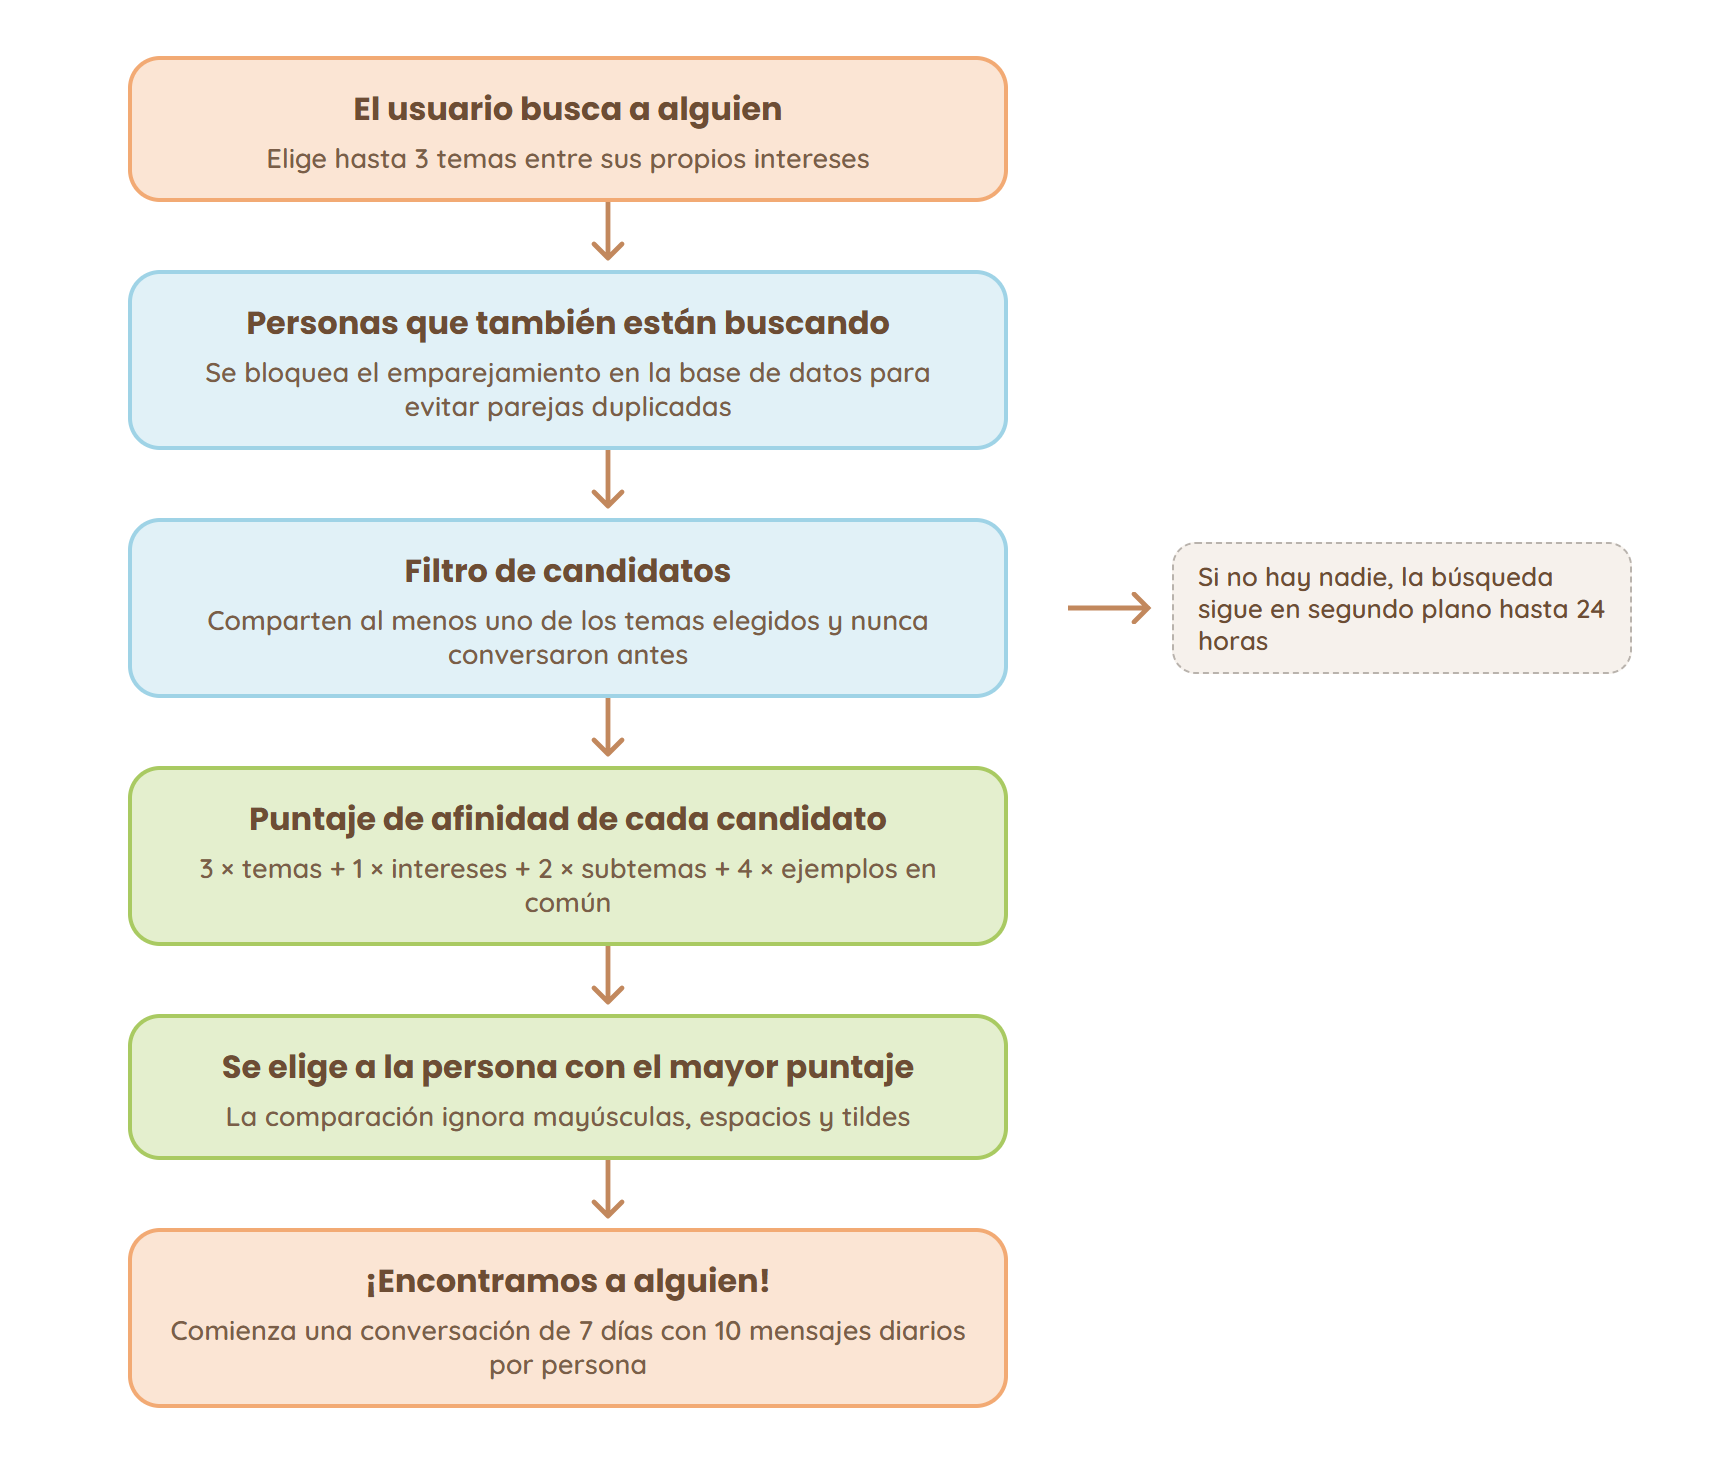
\includegraphics[width=0.75\textwidth]{Images/methodology/prototype/matching.png}
  \vspace{4pt}
\end{figure}

\section{JERARQUÍA DE INTERESES Y AUTOCOMPLETADO}
El catálogo de intereses del prototipo está organizado en 11 categorías y 77 intereses: Entretenimiento, Música, Cultura, Cocina y gastronomía, Bebidas, Deportes, Actividades al aire libre, Estilo de vida, Bienestar, Creatividad, y Social y comunidad. Cada interés cuenta con sus propios subtemas (por ejemplo, Películas tiene géneros, Rock tiene estilos musicales, y Fútbol tiene ligas), y dentro de cada subtema el usuario puede agregar ejemplos concretos de forma opcional (Películas $\rightarrow$ Acción $\rightarrow$ \textit{Iron Man 2}) o de manera general (Películas $\rightarrow$ \textit{Coco}).

Para facilitar el ingreso de ejemplos concretos, la aplicación ofrece autocompletado mediante la Google Knowledge Graph Search API, que sugiere nombres reales filtrados según el tipo de interés (en Películas sugiere únicamente películas; en Rock, bandas y artistas; en Fútbol, equipos y jugadores). El usuario conserva siempre la posibilidad de escribir texto libre si no encuentra el ejemplo que busca. La Figura \ref{fig:autocompletado} muestra las sugerencias que aparecen al escribir una película dentro del subtema Ciencia ficción.

Dado que la API externa responde en aproximadamente un segundo, lo cual excede el Umbral de Doherty de 400 ms que optimiza la productividad percibida (Yablonski, 2020), la interfaz muestra de inmediato las sugerencias ya recibidas que coinciden parcialmente con lo que el usuario va escribiendo, mientras el servidor almacena en caché las respuestas por 24 horas y reutiliza la conexión con el servicio externo, reduciendo así la latencia percibida en búsquedas posteriores. Cuando el servicio externo no encuentra sugerencias, el sistema informa ``Sin sugerencias. Toca + para agregarlo tal como lo escribiste'', atendiendo el principio de retroalimentación, que consiste en comunicar de inmediato al usuario el resultado de sus acciones (Norman, 2013).

\begin{figure}[htbp]
  \centering
  \caption{Autocompletado de gustos específicos en la pantalla ``Cuéntanos más''}
  \label{fig:autocompletado}
  \vspace{4pt}
  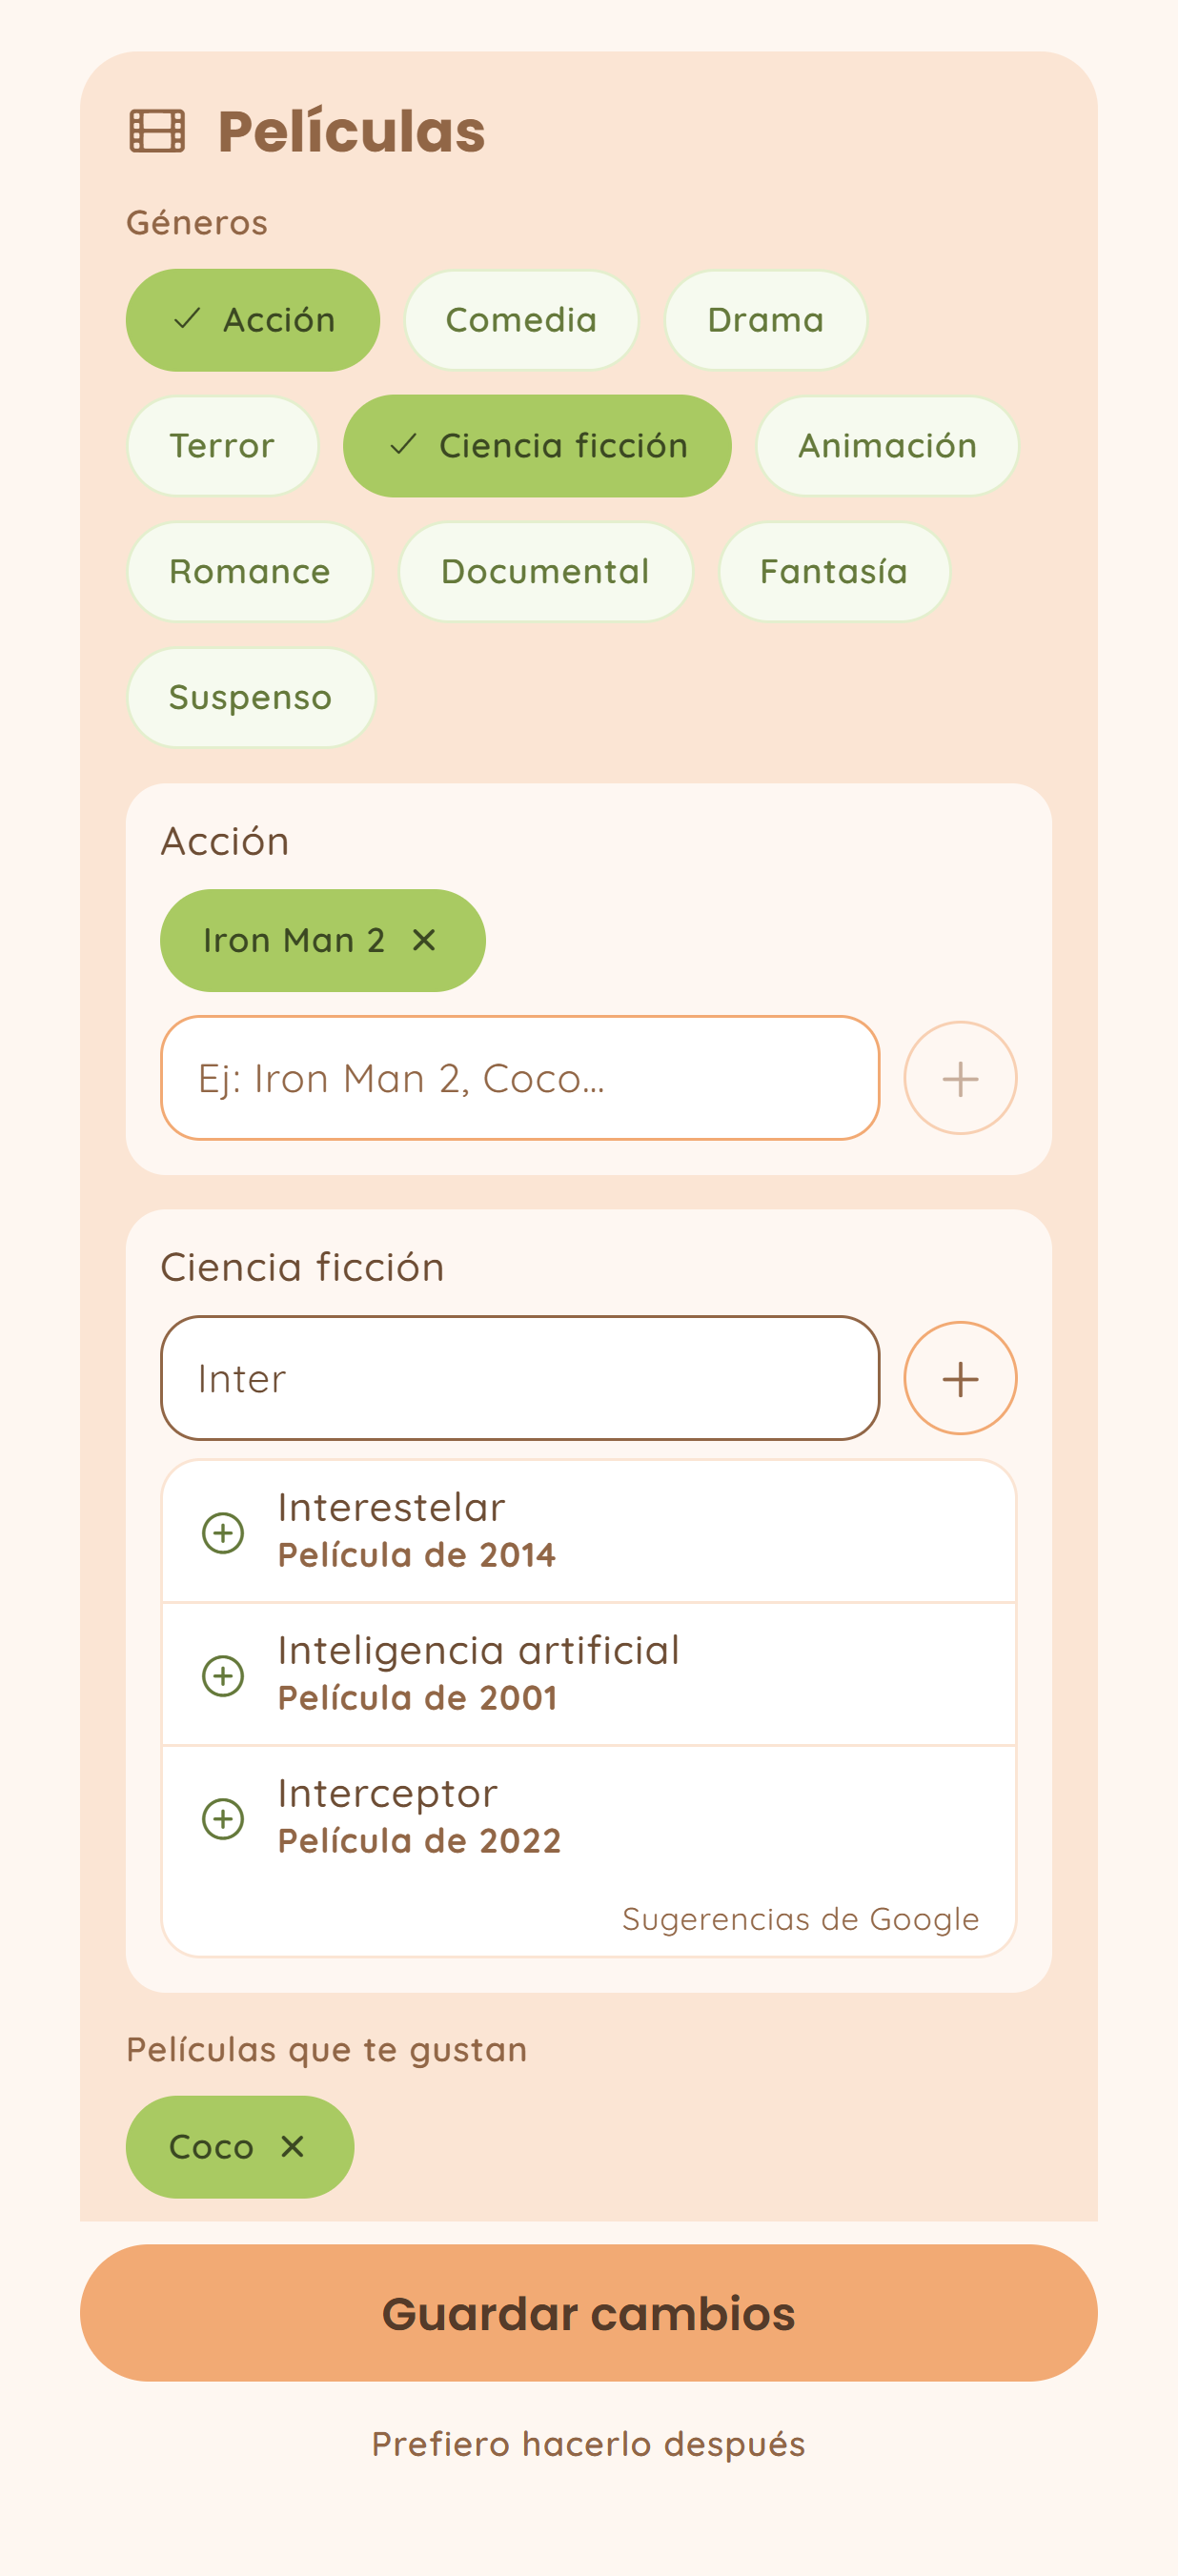
\includegraphics[width=0.42\textwidth]{Images/methodology/prototype/autocomplete.png}
  \vspace{4pt}
\end{figure}

\section{SEGURIDAD Y PRIVACIDAD}
Dado que la aplicación empareja a jóvenes desconocidos entre sí para conversar, se implementaron los siguientes mecanismos de seguridad y protección de la privacidad, en respuesta directa a la necesidad de confianza identificada en la Síntesis de la Fase Empatizar (sección 5.5):

\begin{itemize}
    \item Las contraseñas se almacenan mediante hash Argon2, y se exige un mínimo de 8 caracteres, una mayúscula, un número y un símbolo.
    \item La sesión del usuario se gestiona mediante un token JWT válido por 7 días, almacenado en el almacenamiento seguro del dispositivo.
    \item \textbf{Confirmación del correo.} Al registrarse, el usuario recibe en su correo un código de seis dígitos que debe ingresar en la aplicación. Sin confirmar el correo no es posible buscar pareja, lo cual reduce las cuentas falsas en un espacio donde se conversa con desconocidos.
    \item \textbf{Recuperación de la contraseña mediante código.} La recuperación utiliza el mismo tipo de código, que se ingresa sin salir de la aplicación. Los códigos vencen a los 15 minutos, solo es válido el último solicitado, se anulan tras cinco intentos fallidos y pueden volver a pedirse cada 60 segundos.
    \item Se establece un límite de intentos de inicio de sesión, de recuperación de contraseña y de ingreso de códigos.
    \item La aplicación no solicita fotografías del usuario en ningún momento. El estado de ánimo compartido es opcional, y la decisión final de continuidad de una conversación es privada: un ``no'' de la otra persona no se revela mientras el usuario espera el resultado, evitando así que se infiera el voto ajeno a partir del tiempo de respuesta.
    \item El sistema de reporte permite indicar un motivo (me hizo sentir incómodo/a, contenido ofensivo, acoso o presión, \textit{spam}, otro) junto con un comentario opcional. La conversación se cierra de inmediato y la pareja reportada no vuelve a ser emparejada en el futuro.
    \item Antes de usar la aplicación, el usuario lee y acepta los acuerdos de convivencia, descritos a continuación.
\end{itemize}

\subsection{Acuerdos de convivencia}
Los acuerdos se presentan en la pantalla ``Un lugar seguro'' del \textit{onboarding} y pueden consultarse en cualquier momento desde Ajustes. Están redactados en segunda persona y en frases breves, y se organizan en cinco apartados:

\begin{itemize}
    \item \textbf{Cómo funciona ECHOOM:} el usuario elige hasta tres temas entre sus intereses y se le presenta a una persona que comparte al menos uno; ambos tienen siete días para conocerse, con diez mensajes al día cada uno, y las reacciones no cuentan como mensaje; la planta crece cada día en que los dos se escriben; desde el día 7 disponen de tres días para decidir en privado si desean seguir en contacto, y la conversación continúa solo si ambos aceptan; además, nunca se vuelve a presentar a dos personas que ya conversaron.
    \item \textbf{Tu cuenta:} se requiere tener 16 años o más, confirmar el correo con un código de seis dígitos para poder buscar a alguien, y no compartir la contraseña, que se almacena cifrada.
    \item \textbf{Para cuidarnos entre todas las personas:} se pide tratar a los demás con respeto, sin acoso, odio, amenazas ni contenido ofensivo; se informa que cada mensaje se revisa antes de enviarse (sección 8.5.2), que no se permiten nombres de usuario ofensivos y que es posible salir de una conversación o reportarla en cualquier momento, sin que la otra persona vea el motivo.
    \item \textbf{Tu privacidad:} no se solicitan fotografías; el historial de ánimo es privado y la otra persona solo ve el ánimo de las últimas 24 horas en el avatar, lo cual puede desactivarse; la decisión final es privada; se detallan los datos que se almacenan (nombre de usuario, correo, avatar, intereses, registros de ánimo y mensajes), que se usan únicamente para el funcionamiento de la aplicación y no con fines publicitarios; se advierte que el texto que se escribe al describir los gustos se consulta a Google para sugerir nombres, sin el nombre ni el correo del usuario; y, dado que no se verifican identidades, se recomienda no compartir datos personales como la dirección o el teléfono.
    \item \textbf{Un espacio que acompaña:} se aclara que ECHOOM no reemplaza la ayuda profesional y se recomienda acudir a alguien de confianza o a un servicio de ayuda en un momento difícil, en línea con los límites definidos en la sección 1.5 del presente documento.
\end{itemize}

Para continuar, el usuario marca la casilla ``Leí y acepto estos acuerdos, incluido el uso de mis datos''. Explicitar qué datos se guardan y con qué fin responde a la necesidad de protección de la privacidad frente a desconocidos identificada en la fase de Definir (Capítulo 6). La Figura \ref{fig:seguridad} muestra los acuerdos de convivencia y la pantalla en la que se ingresa el código enviado al correo.

\begin{figure}[htbp]
  \centering
  \caption{Acuerdos de convivencia y confirmación del correo}
  \label{fig:seguridad}
  \vspace{4pt}
  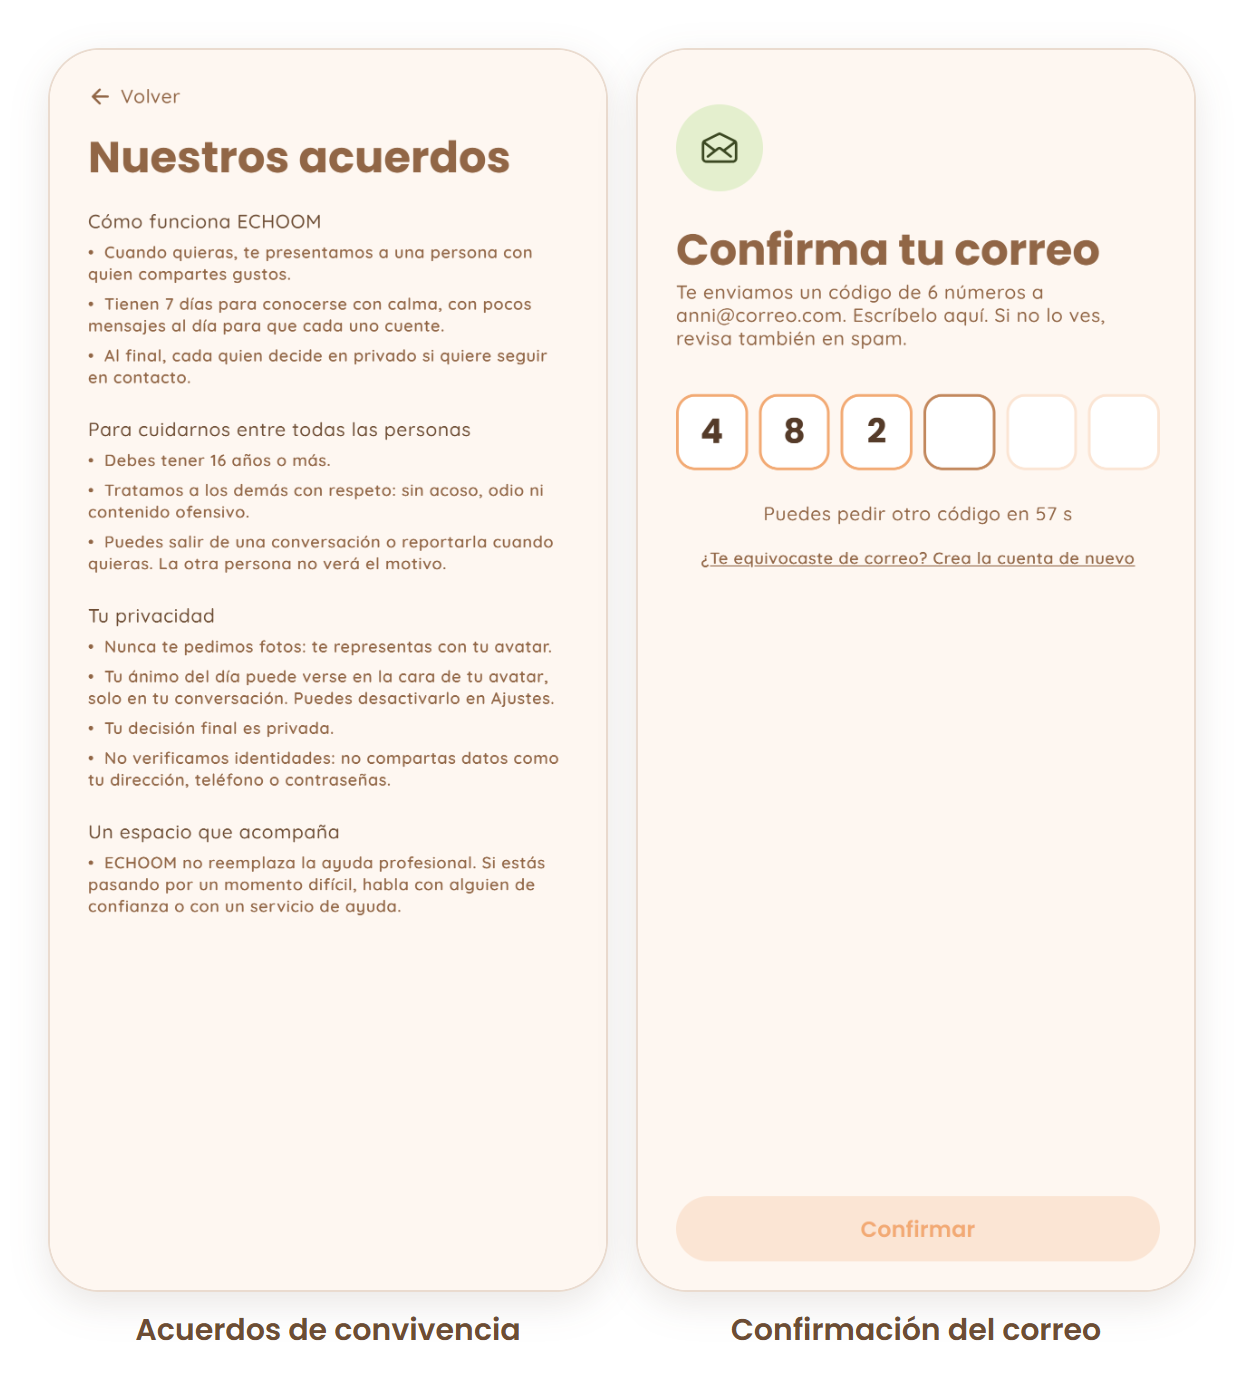
\includegraphics[width=0.7\textwidth]{Images/methodology/prototype/security.png}
  \vspace{4pt}
\end{figure}

\subsection{Moderación antes de enviar}
El objetivo general del proyecto habla de micro interacciones sociales \textit{positivas}. Para resguardar ese carácter, cada mensaje pasa por una moderación de dos niveles que lo analiza en el servidor antes de guardarlo, de modo que la regla no puede evitarse desde la aplicación:

\begin{itemize}
    \item \textbf{Nivel leve} (tono brusco o burlas): aparece una pausa amable, ``¿Lo reformulamos?'', que muestra el mensaje y ofrece las opciones \textit{Editar mensaje} o \textit{Enviar igual}. No castiga, sino que invita a reconsiderar.
    \item \textbf{Nivel grave} (insultos fuertes, amenazas, acoso sexual o incitación a la autolesión): el mensaje no se envía, se informa que ``no cuida a la otra persona'' y el texto vuelve al campo para reformularlo, sin descontar del límite diario.
\end{itemize}

Este diseño se apoya en el experimento de Katsaros et al. (2022), en el que una pausa antes de publicar llevó a cancelar el 9~\% y a modificar el 22~\% de los mensajes ofensivos, y redujo el contenido ofensivo publicado posteriormente. Desde la regulación emocional, la pausa ayuda a frenar la respuesta impulsiva antes de que ocurra (Gross, 1998), y desde la usabilidad corresponde a la prevención de errores (Shneiderman et al., 2016). El detector reconoce disfraces comunes, como letras separadas, números en lugar de letras, signos entre letras y letras repetidas, y evita falsos positivos con palabras inocentes; además, se rechazan los nombres de usuario ofensivos. Como limitación, se trata de una lista de expresiones en español y no de un modelo que comprenda el contexto, por lo que puede no detectar ofensas nuevas o muy sutiles. Los clasificadores automáticos disponibles se descartaron en esta etapa: el de Google Cloud Natural Language requiere una cuenta de facturación, y Perspective API anunció su cierre para finales de 2026. Un clasificador automático queda como trabajo futuro.

La Figura \ref{fig:moderacion} muestra ambos niveles de la moderación dentro de la conversación.

\begin{figure}[htbp]
  \centering
  \caption{Moderación antes de enviar en sus dos niveles}
  \label{fig:moderacion}
  \vspace{4pt}
  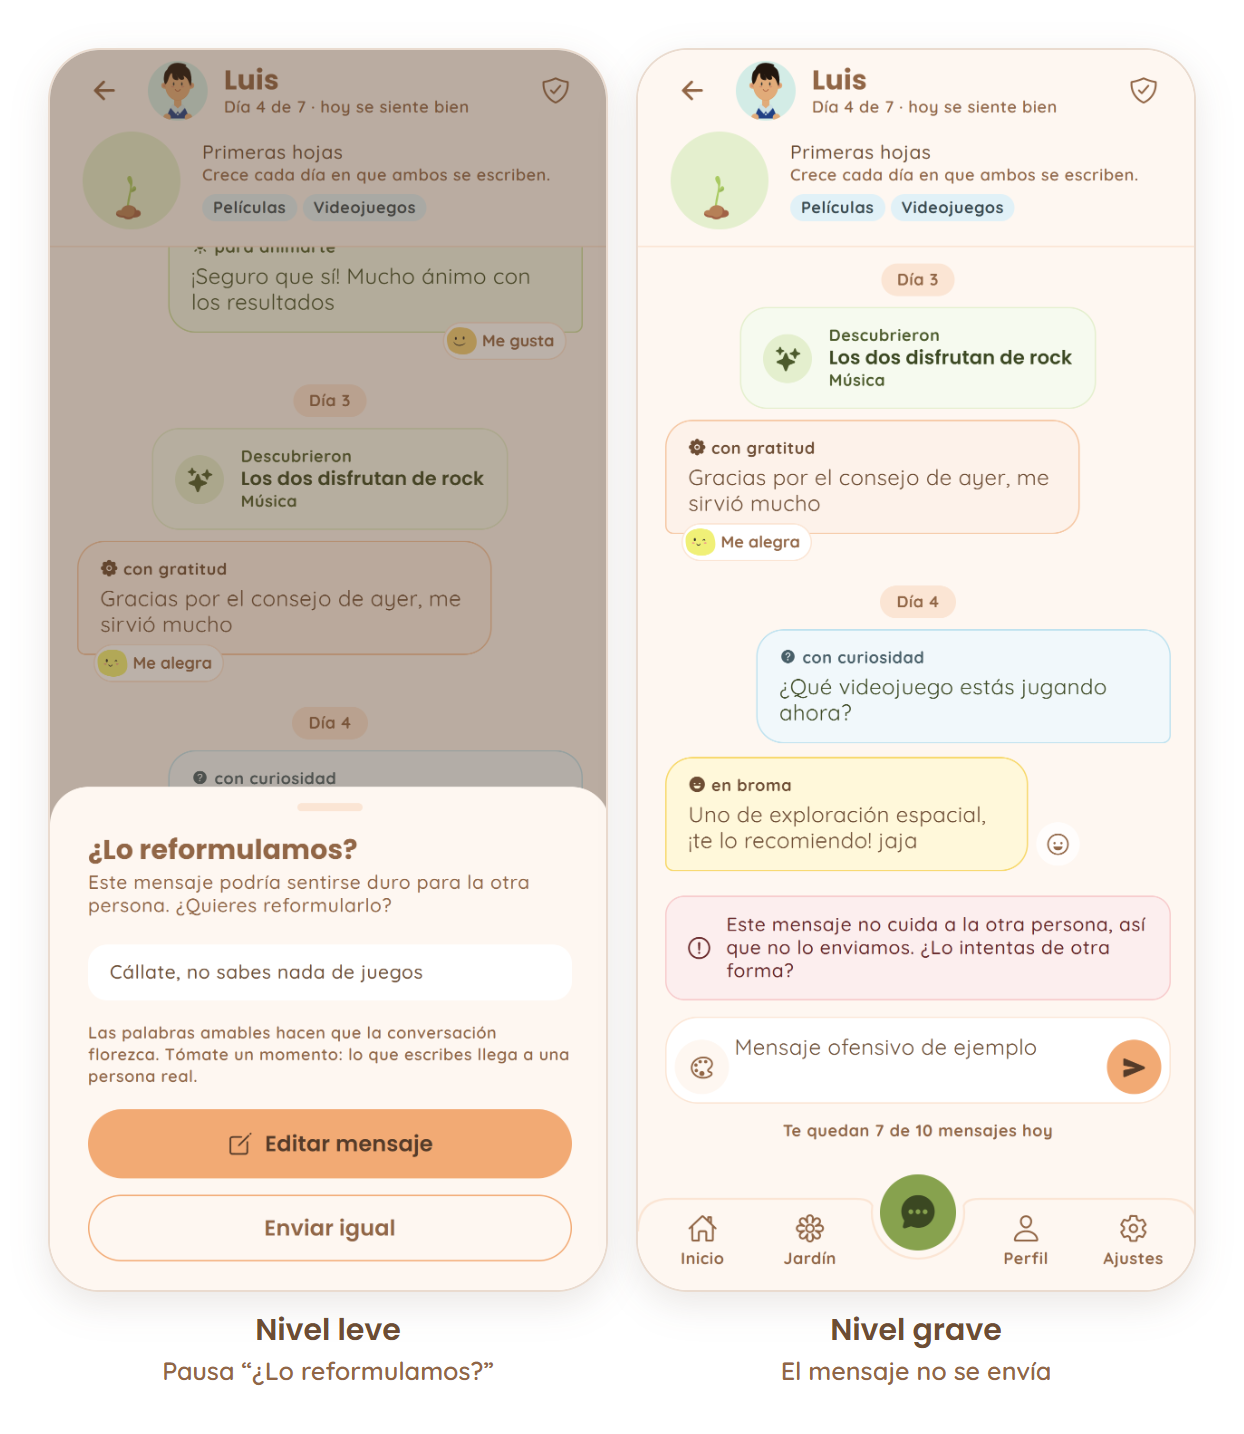
\includegraphics[width=0.7\textwidth]{Images/methodology/prototype/moderation.png}
  \vspace{4pt}
\end{figure}

\section{SISTEMA DE DISEÑO: IHC AFECTIVA Y UX/UI EMOCIONAL}
El sistema de diseño del prototipo se construyó deliberadamente para traducir en elementos visuales e interactivos concretos los principios de IHC Afectiva revisados en el Capítulo 2, evitando los códigos visuales que la literatura del Capítulo 4 asocia a la ansiedad social y la comparación: colores de alerta, contadores públicos y notificaciones de enganche.

\subsection{Paleta de colores y accesibilidad}
La paleta es cálida y natural, compuesta por un color durazno como color principal, verde para representar el crecimiento y las acciones positivas, y celeste para transmitir calma y acceso a la ayuda, complementada con cinco colores adicionales utilizados en la representación de los estados de ánimo (Figura \ref{fig:paleta}). La gama de rojos se reserva para los errores y las acciones delicadas, como salir de una conversación o reportarla. Cada color cuenta con diez tonos, del más claro al más oscuro, y junto a cada uno se indica su contraste con el texto negro y blanco.

\begin{figure}[htbp]
  \centering
  \caption{Paleta de colores de ECHOOM y contraste de cada tono}
  \label{fig:paleta}
  \vspace{4pt}
  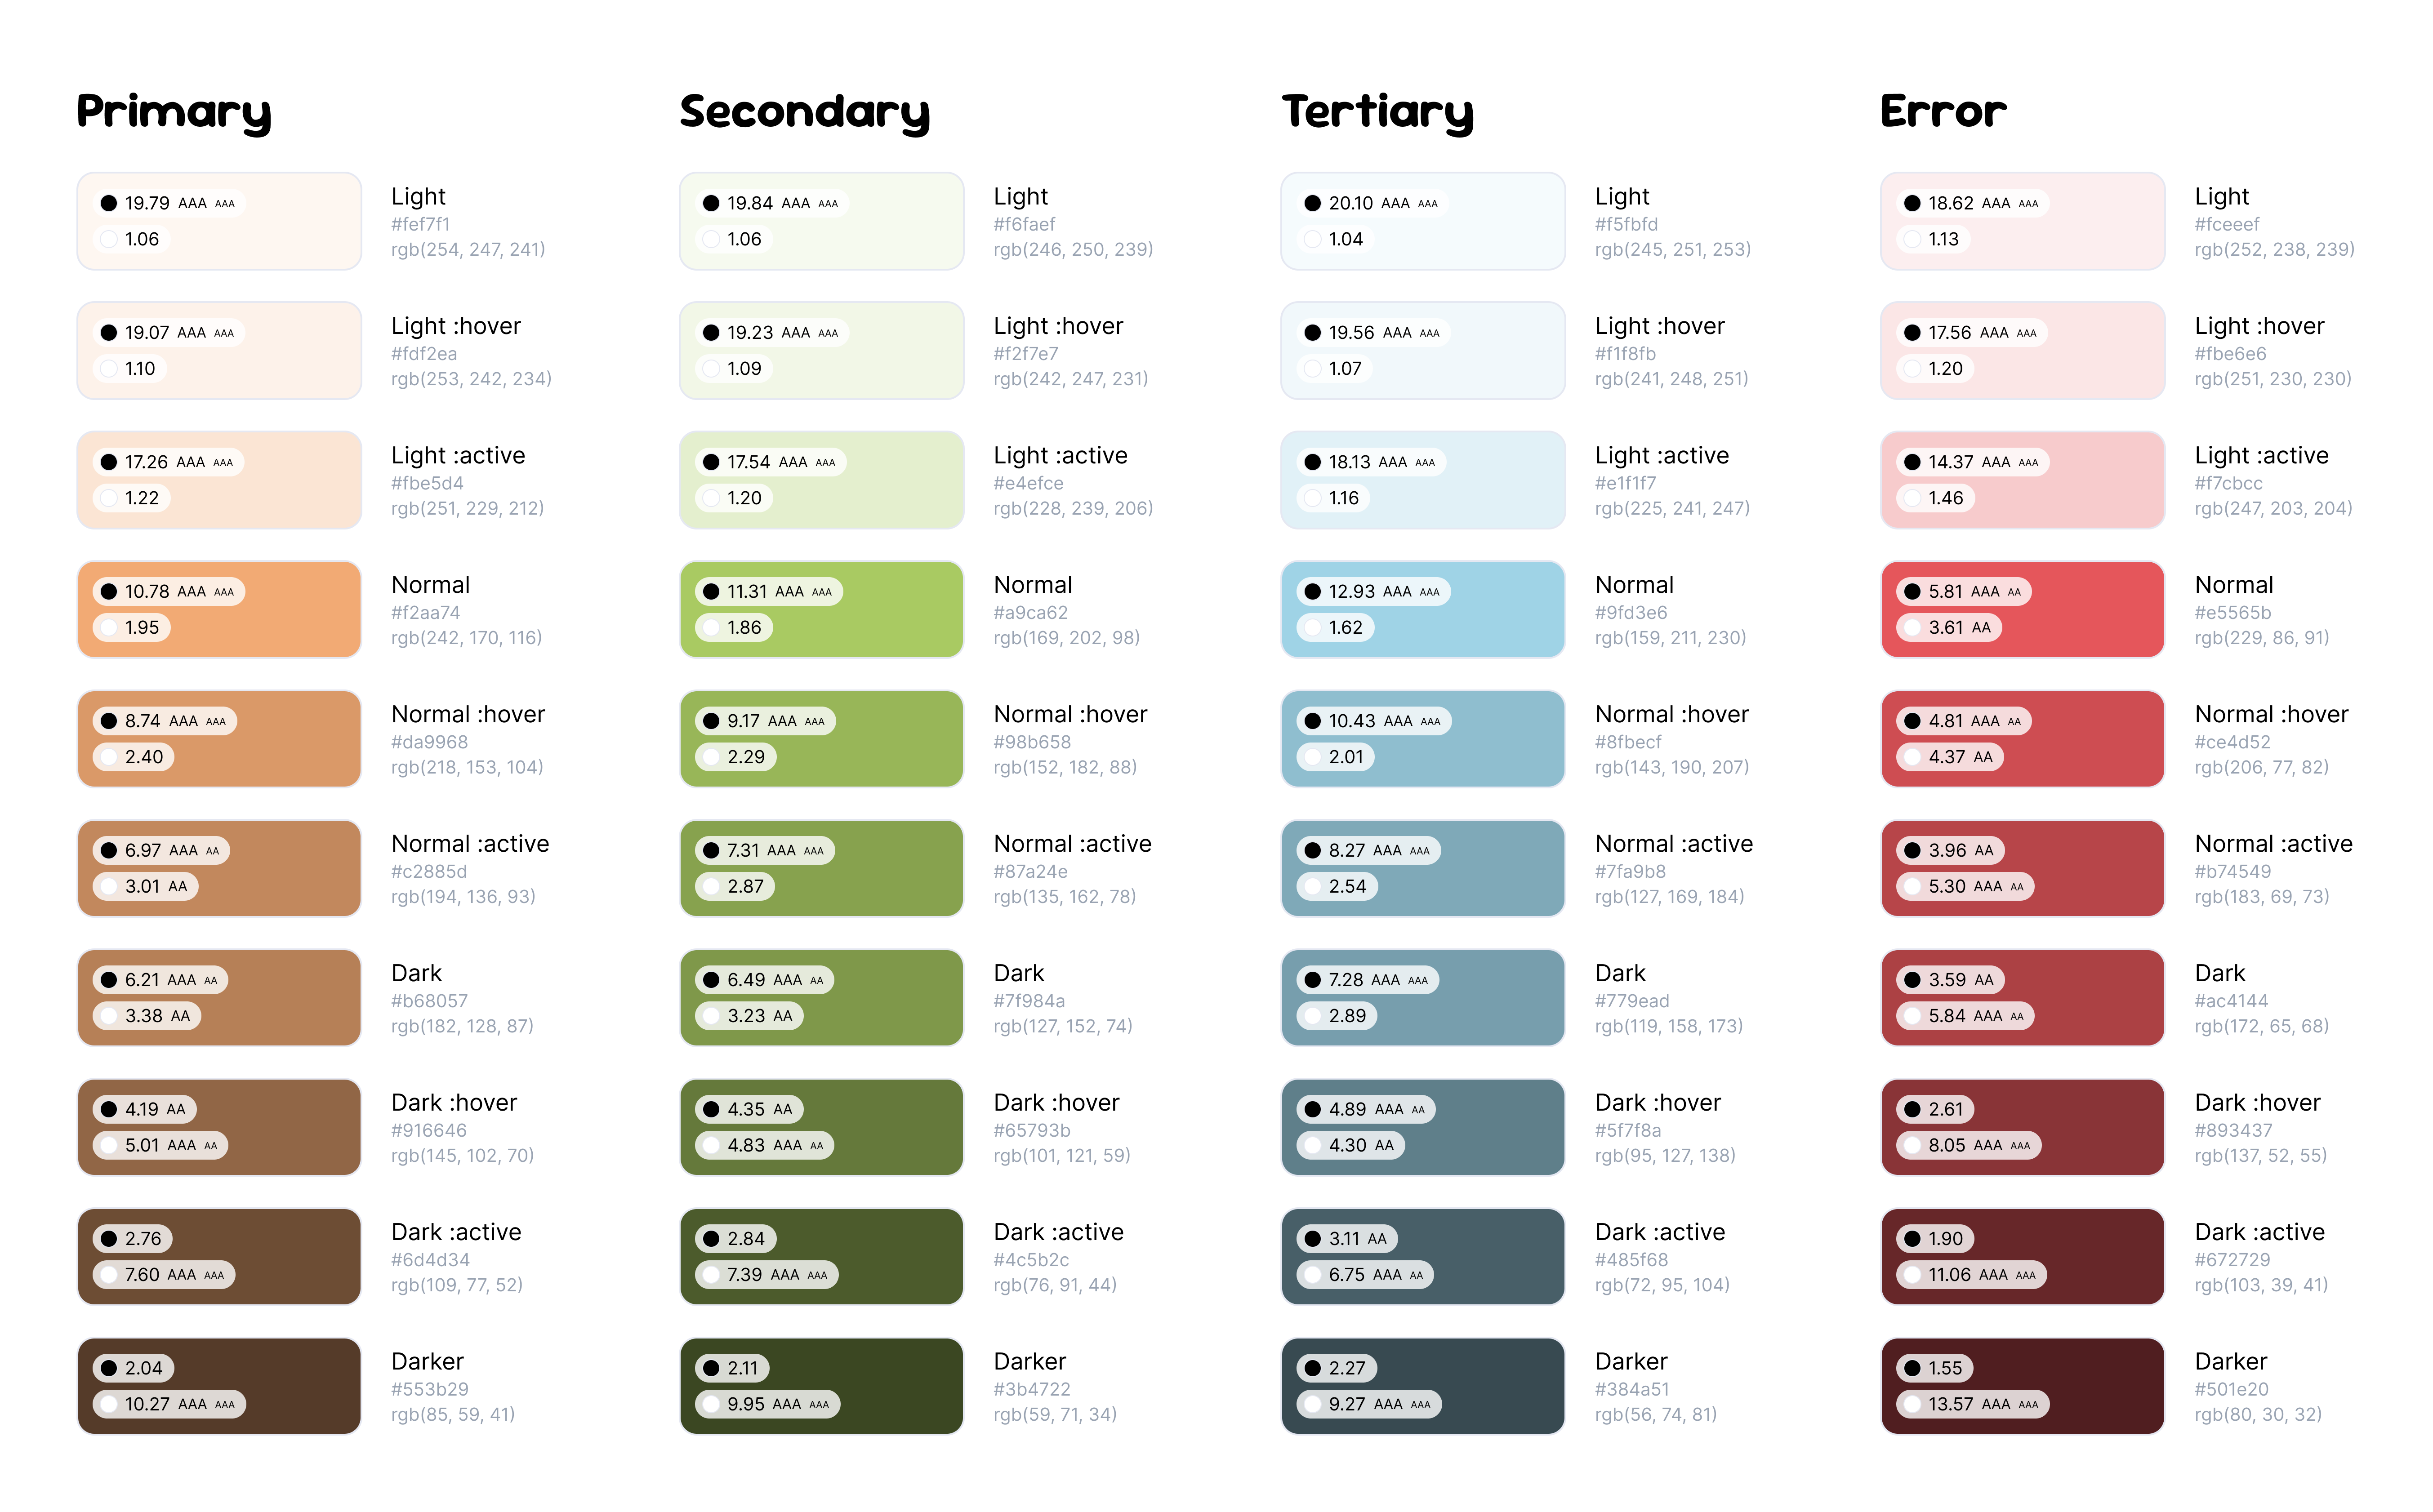
\includegraphics[width=0.95\textwidth]{Images/methodology/prototype/colors.png}
  \vspace{4pt}
\end{figure}

Dado que la calidez cromática por sí sola no garantiza la legibilidad, el contraste de todos los elementos de texto e interactivos se midió conforme a las Pautas de Accesibilidad para el Contenido Web (WCAG) 2.2 (W3C, 2023), y para cada uno se eligieron, dentro de la misma paleta, los tonos que alcanzan el mínimo recomendado. La Tabla \ref{tab:contraste} resume el contraste de los elementos principales.

\begin{longtable}{
  >{\raggedright\arraybackslash}p{0.34\textwidth}
  >{\raggedright\arraybackslash}p{0.36\textwidth}
  >{\centering\arraybackslash}p{0.2\textwidth}
}
\caption{Contraste de los elementos principales según WCAG 2.2}\label{tab:contraste}\\
\toprule
\textbf{Elemento} & \textbf{Combinación} & \textbf{Contraste} \\
\midrule
\endfirsthead
\multicolumn{3}{l}{\textit{Tabla \thetable{} (continuación)}} \\[4pt]
\toprule
\textbf{Elemento} & \textbf{Combinación} & \textbf{Contraste} \\
\midrule
\endhead
\midrule
\multicolumn{3}{r}{\textit{Continúa en la siguiente página}} \\
\endfoot
\bottomrule
\endlastfoot

Botón principal & Café oscuro sobre durazno & 5,27:1 \\
Botones verdes y celestes & Tono más oscuro de cada color sobre su fondo & 5,30:1 y 5,71:1 \\
Enlaces y texto & Cafés de la paleta sobre fondos claros & 4,72:1 -- 7,17:1 \\
Títulos y subtítulos (texto grande) & Café cálido (\#916646) sobre los fondos de la aplicación & 4,1:1 o más \\
Saludo de Inicio & Café \#6D4D34 sobre la ilustración de la colina & 4,5:1 \\

\end{longtable}

\noindent\textit{Nota.} Elaboración propia.

Adicionalmente, todos los objetivos táctiles de la interfaz miden al menos entre 40 y 48 px, conforme a la Ley de Fitts, que establece que el tiempo requerido para alcanzar un objetivo es función de su tamaño y distancia (Yablonski, 2020). Ningún estado depende únicamente del color: la pestaña activa cambia su ícono de contorno a relleno, y la emoción elegida, además de quedar sobre un círculo de su color, aumenta de tamaño y oscurece su nombre (W3C, 2023, criterio 1.4.1).

\subsection{Tipografía}
Se utiliza Poppins para los títulos y Quicksand para el cuerpo de texto, organizadas en una escala tipográfica Major Second (1,125) con un tamaño mínimo de 12 px en toda la interfaz (Figura \ref{fig:tipografia}). Esta combinación tipográfica, de formas redondeadas, refuerza la calidez emocional de la aplicación en coherencia con la faceta de lo deseable propuesta por Morville (2005, como se citó en Méndez et al., 2014), evitando las fuentes geométricas y frías asociadas a interfaces de carácter corporativo.

\begin{figure}[htbp]
  \centering
  \caption{Escala tipográfica de ECHOOM}
  \label{fig:tipografia}
  \vspace{4pt}
  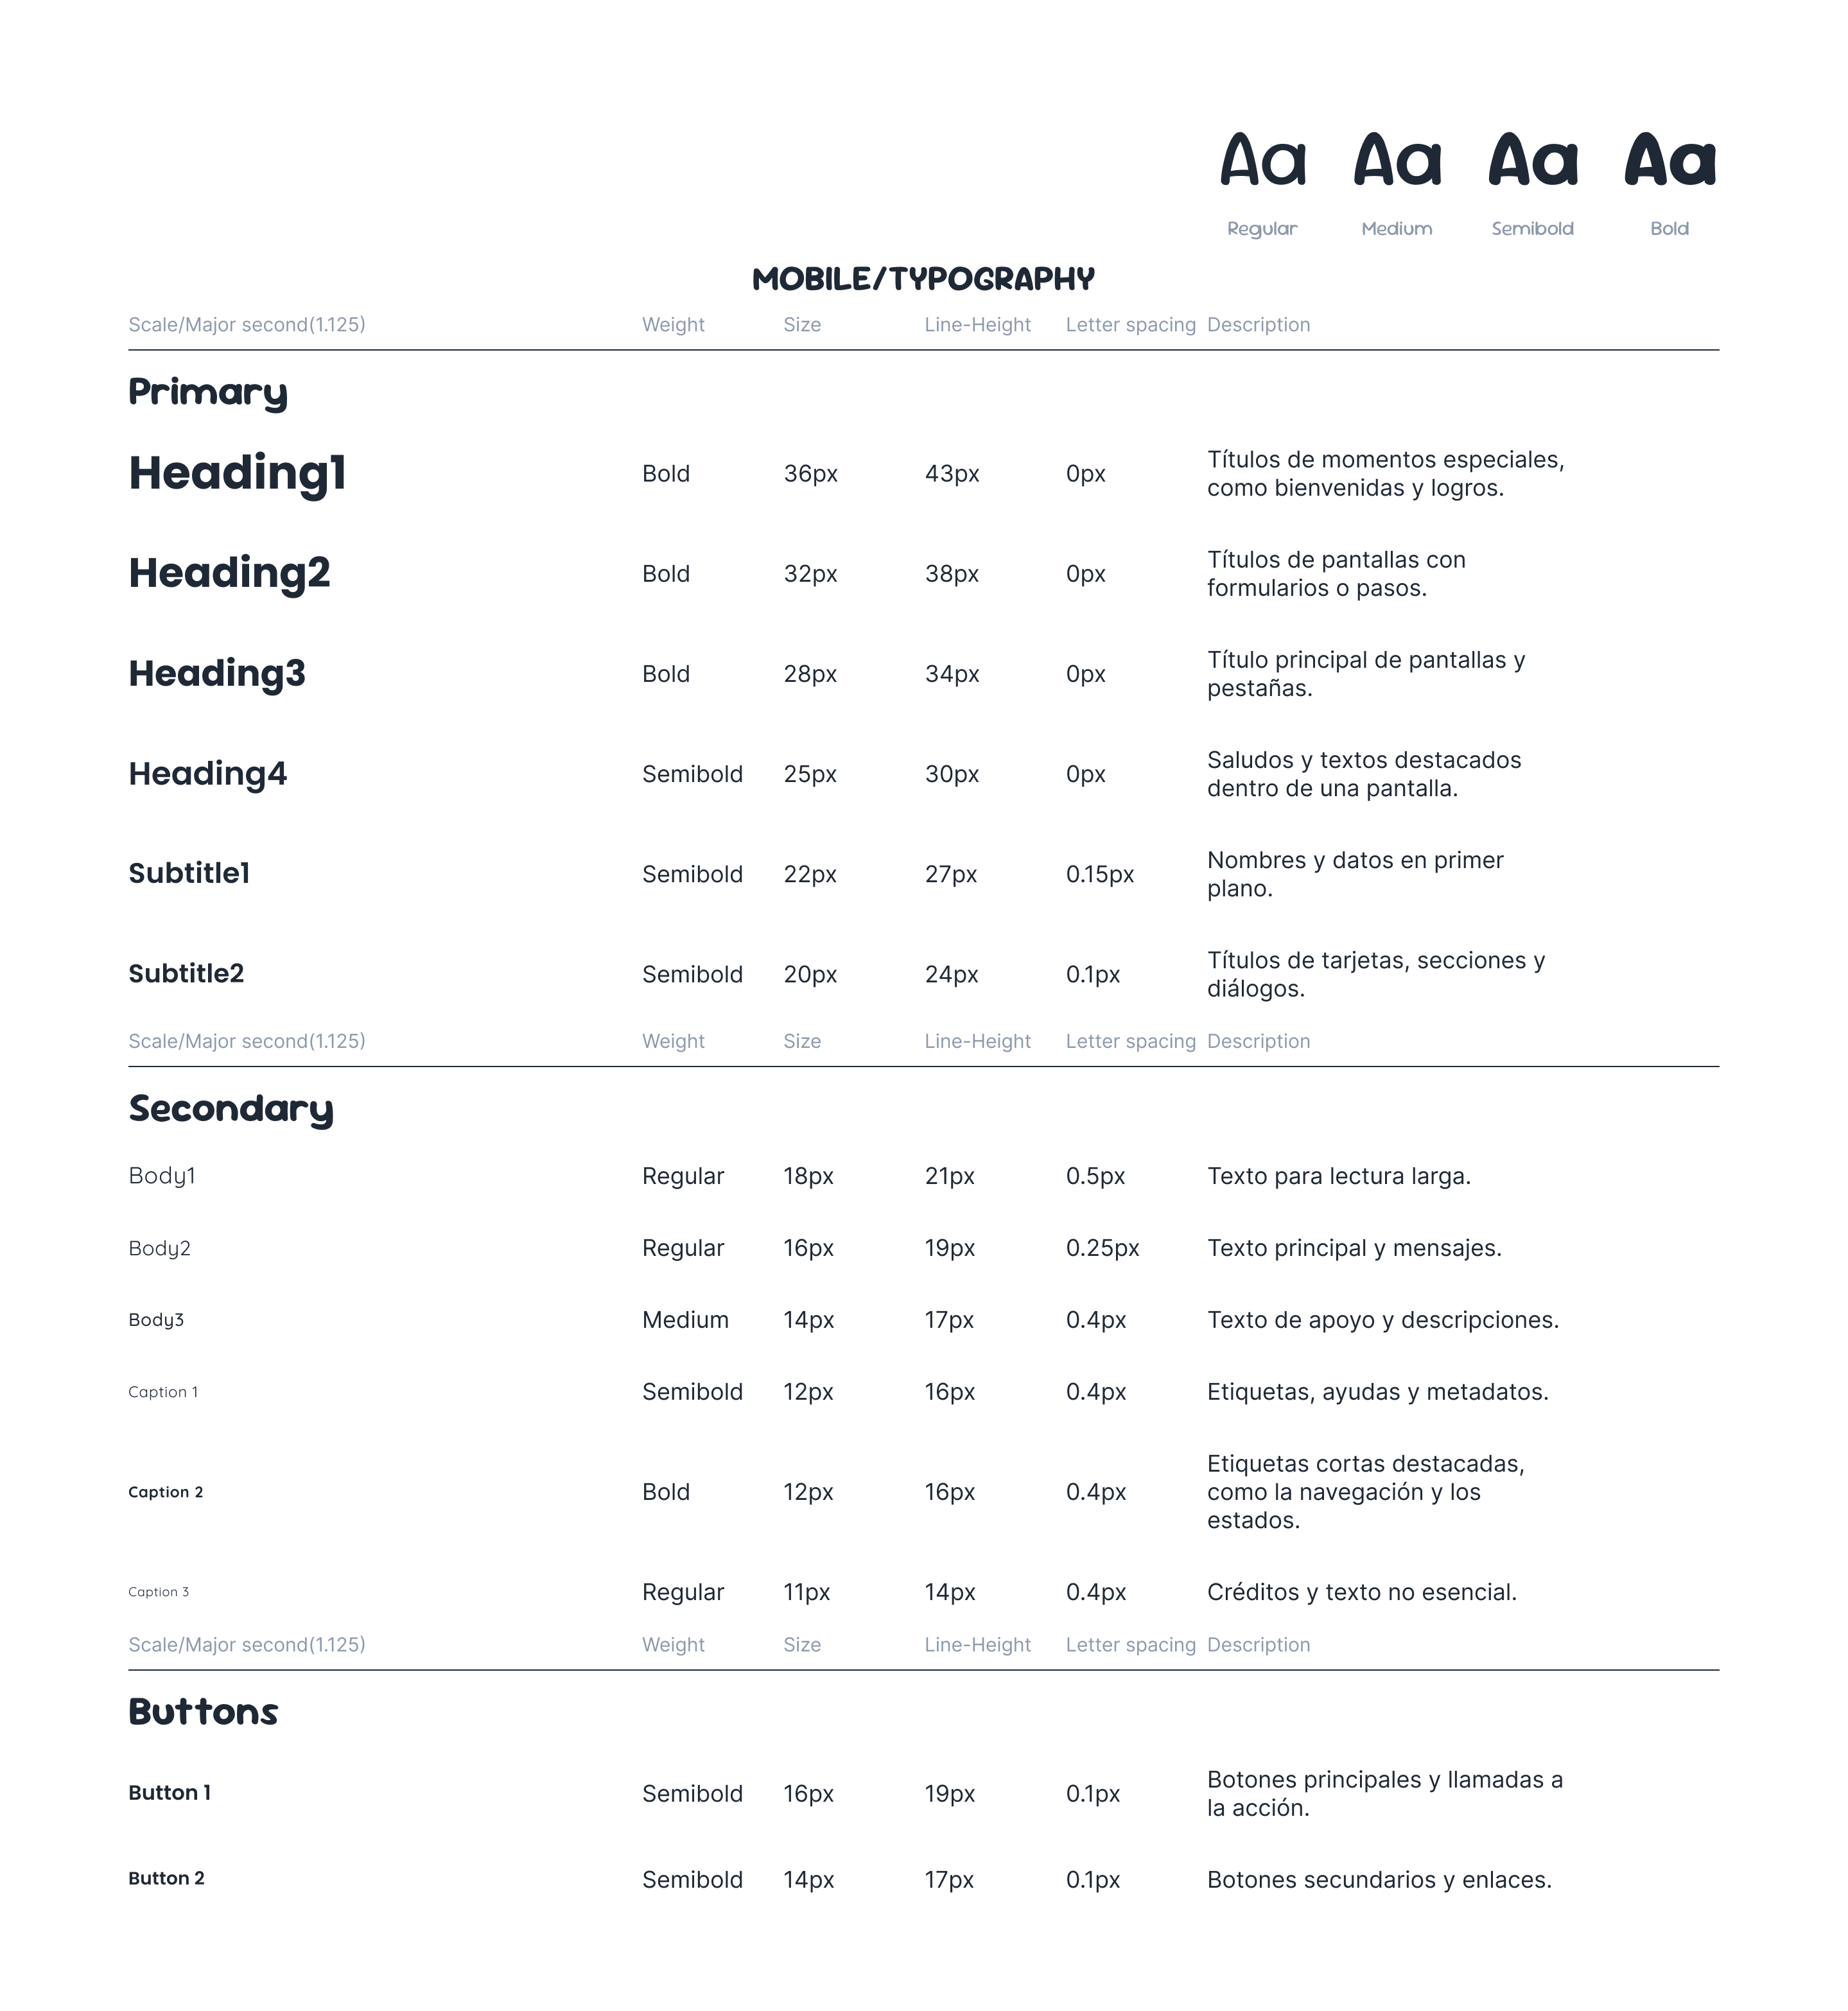
\includegraphics[width=0.85\textwidth]{Images/methodology/prototype/typography.png}
  \vspace{4pt}
\end{figure}

Cada nivel de la escala tiene un uso definido: Heading 1 (36 px) marca los momentos de llegada, como el nombre del usuario en la bienvenida; Heading 3 (28 px) titula las pantallas y pestañas; y Subtitle 2 (20 px) titula tarjetas, secciones y diálogos. Los títulos y subtítulos utilizan un café cálido de la paleta (\#916646, el mismo del logo), y el texto, un café más profundo (\#6D4D34). En el prototipo, los subtítulos y los saludos se presentan en negrita, de modo que, conforme a WCAG 2.2, cuentan como texto grande y requieren un contraste de 3:1; el café cálido alcanza 4,1:1 o más sobre todos los fondos utilizados. Se eligió el tono más claro que aún cumple este criterio, en busca de una lectura más cálida (nivel visceral del diseño emocional; Norman, 2004); el saludo de Inicio, que se ubica sobre la ilustración de la colina, utiliza el tono siguiente de la escala para mantener el contraste.

\subsection{Ilustraciones propias}
Con el fin de construir una identidad visual propia y coherente, la autora diseñó ilustraciones originales en formato vectorial (SVG), que se animan por partes dentro de la aplicación:

\begin{itemize}
    \item Una \textbf{semilla de bienvenida}, que llega con sus hojas, saluda con ellas, parpadea y flota antes de que aparezca el texto ``Te damos la bienvenida''. Es el primer momento de cada sesión, por lo que se cuidó especialmente (Regla del Pico-Final; Yablonski, 2020).
    \item Cinco \textbf{caras de ánimo} (fatal, mal, normal, bien y feliz), que expresan su emoción todo el tiempo: feliz da saltitos, bien se mece y sonríe, normal mira a los lados, mal suspira y fatal se balancea despacio con los ojos bajos. Todas parpadean y reaccionan al ser elegidas.
    \item Una \textbf{planta en siete etapas}, una por cada día de la semana, desde la semilla hasta la flor completa. Cada etapa nueva crece desde la tierra con un pequeño rebote, y al abrir la conversación o el jardín la planta recorre sus etapas como un \textit{time-lapse}.
    \item El \textbf{fondo de Inicio}, con cielo, nubes, una montaña, un árbol y hierba, que se adapta a cualquier ancho de pantalla sin deformarse y se mueve con suavidad: las nubes van y vienen, la hierba se mece y la montaña se desplaza despacio, mientras el árbol y el suelo permanecen quietos para que el contenido se apoye sobre algo estable.
    \item Los \textbf{paisajes} de la pantalla diaria de la planta y del jardín, con nubes, sol y colinas que se mecen, y \textbf{mariposas} que recorren el jardín.
\end{itemize}

Todo el movimiento es lento y periférico, para informar sin reclamar atención, conforme al principio de tecnología calmada (Weiser \& Brown, 1996), y se detiene cuando el usuario activa la opción ``Reducir movimiento'' de su dispositivo (W3C, 2023, criterio 2.3.3).

La Figura \ref{fig:ilustraciones} reúne estas ilustraciones.

\begin{figure}[htbp]
  \centering
  \caption{Ilustraciones propias de ECHOOM}
  \label{fig:ilustraciones}
  \vspace{4pt}
  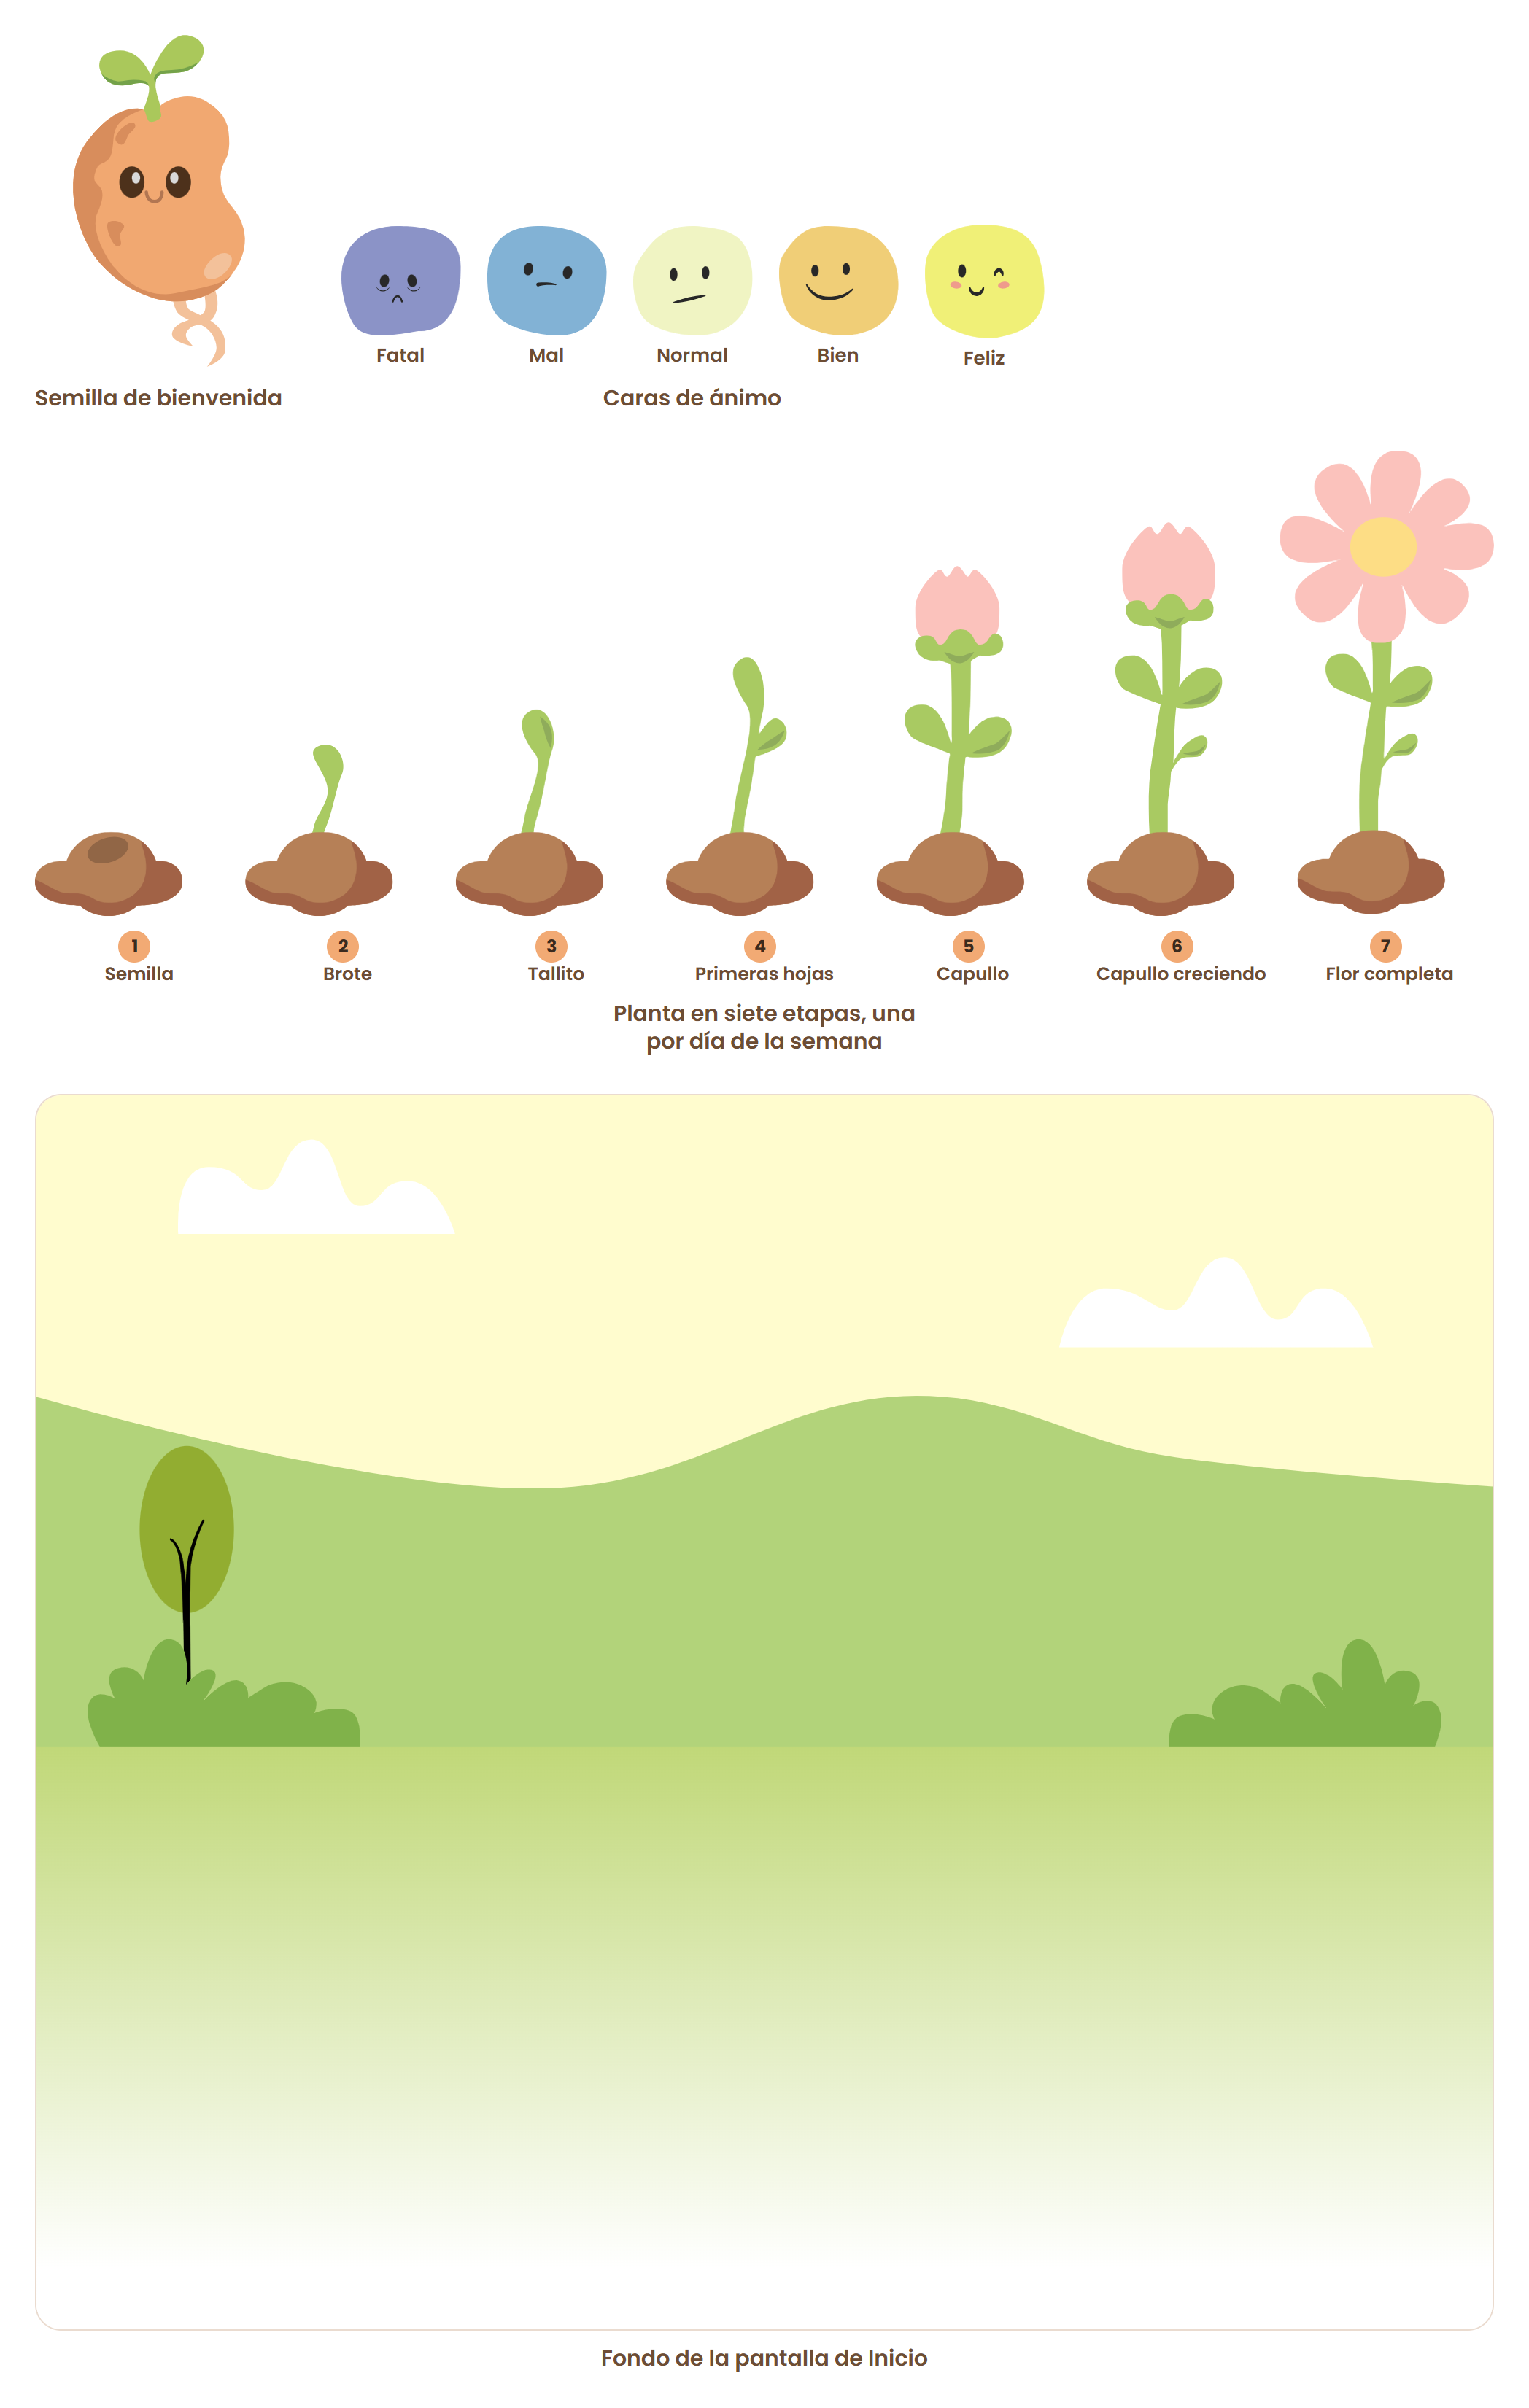
\includegraphics[width=0.72\textwidth]{Images/methodology/prototype/illustrations.png}
  \vspace{4pt}
\end{figure}

\subsection{Avatar ilustrado y avatar vivo}
El avatar fue dibujado por la autora y se arma por capas. Primero se elige ``Chica'' o ``Chico'', lo que determina los peinados, flequillos, prendas y barbas disponibles: para chica, 12 peinados, 9 flequillos, 3 tipos de aretes, diadema y 7 prendas; para chico, 9 peinados más la opción sin cabello, 10 flequillos, 4 barbas y 7 prendas. Ambos comparten 6 tonos de piel, 6 colores de cabello, 3 tipos de lentes, pecas, lunar, 8 colores de ropa y un color de fondo. Cada opción se muestra como una miniatura del propio avatar con esa opción aplicada, lo que permite reconocer en lugar de recordar (Nielsen, como se citó en Hernández Bieliukas, 2014), y las opciones se organizan en una cuadrícula de cuatro columnas para que sean fáciles de ver y de tocar (Ley de Fitts; Yablonski, 2020). La expresión del avatar refleja el ánimo del día: los ojos y la boca cambian según la emoción registrada, y en los tonos de piel más oscuros la boca y los ojos usan tonos más profundos para que la emoción se distinga incluso en tamaños pequeños.

Además, el avatar \textbf{cobra vida}: respira, parpadea y se mece según su ánimo (con ánimo feliz da pequeños saltos; con ánimo bajo respira más lento). Saluda inclinando el cuerpo y moviendo la mano, representada como una pequeña esfera sin brazos, tal como fue dibujada; celebra con las dos manos a la altura de los hombros y asiente. En la pantalla de Inicio saluda al entrar y al ser tocado, y reacciona al ánimo registrado: celebra si es ``feliz'', saluda si es ``bien'' y asiente si es ``normal''; con ánimo bajo no celebra ni sonríe a la fuerza, para no invalidar la emoción. La otra persona saluda al encontrarse por primera vez y celebra cuando la planta florece. Un personaje que responde con expresiones y gestos sociales transmite presencia y genera mayor agrado (efecto de persona; Lester et al., 1997). Para que estos movimientos no dejen ver huecos, la ropa de los avatares llega hasta la línea inferior y cubre todo el ancho del cuerpo, siguiendo el principio de ``dibujo sólido'' de la animación (Thomas \& Johnston, 1981).

La Figura \ref{fig:avatar} muestra el editor del avatar y tres de sus gestos: reposo, saludar y celebrar.

\begin{figure}[htbp]
  \centering
  \caption{Editor del avatar y gestos del avatar vivo}
  \label{fig:avatar}
  \vspace{4pt}
  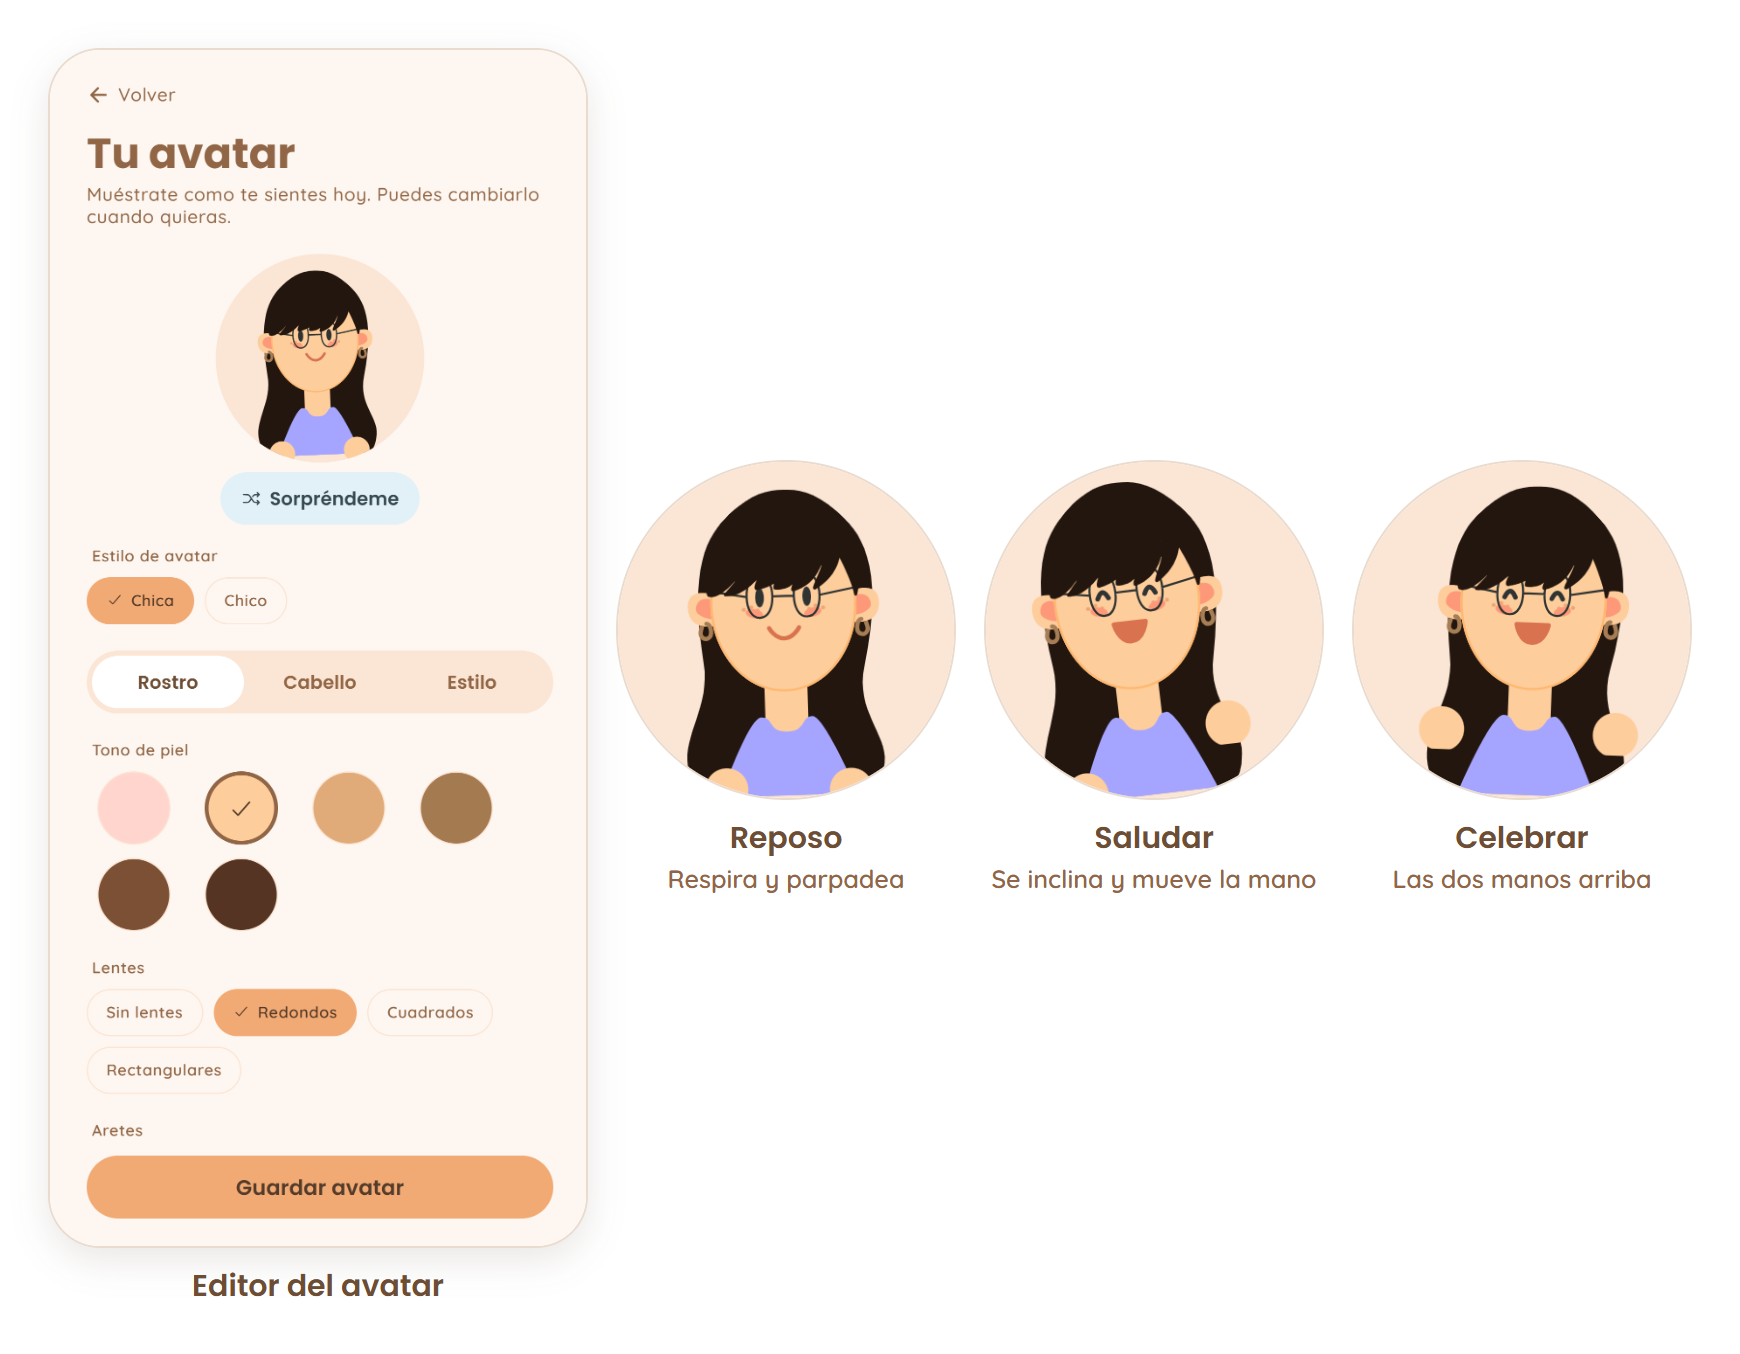
\includegraphics[width=\textwidth]{Images/methodology/prototype/avatar.png}
  \vspace{4pt}
\end{figure}

\subsection{Registro del ánimo}
La primera vez de cada día, antes de entrar a Inicio, una pantalla sobre un paisaje con sol pregunta ``¿Cómo te sientes hoy?'', con la opción ``Ahora no'' para omitirla. El ánimo puede actualizarse durante el día, y la tarjeta ``Tu día'' muestra el historial de la jornada como una cinta de colores, un tramo por registro, y una línea de tiempo con la cara, el nombre y la hora de cada registro. Registrar el ánimo varias veces al día permite captar cómo cambia, de forma similar al muestreo ecológico momentáneo (Shiffman et al., 2008), y ponerle nombre a la emoción ya contribuye a regularla (Lieberman et al., 2007). Omitir el registro siempre es posible, en respeto de la autonomía del usuario (Peters et al., 2018), y el historial es privado y no incluye cifras ni rachas.

Dado que los registros no pueden borrarse, al tocar una cara se abre una confirmación (``¿Así te sientes?'', con las opciones ``Sí, guardar'' y ``Elegir otra''), conforme a los principios de prevención de errores y de control y libertad del usuario (Nielsen, como se citó en Hernández Bieliukas, 2014).

Cuando el ánimo registrado es ``mal'' o ``fatal'', se abre una pantalla de respiración guiada antes de continuar: tres respiraciones lentas (4 segundos al inhalar y 6 al exhalar, unos 30 segundos en total), representadas por un círculo en el color de la emoción que crece al inhalar y se encoge al exhalar, mientras la cara de la emoción respira con el usuario y, al exhalar, ondas suaves se alejan y se desvanecen. La respiración lenta reduce la activación fisiológica y la ansiedad (Lehrer \& Gevirtz, 2014; Zaccaro et al., 2018), y realizarla antes de entrar a la conversación es una estrategia de regulación previa a la respuesta (Gross, 1998), para no escribir a la otra persona desde el malestar. El ejercicio puede omitirse en cualquier momento, y al finalizar pregunta de forma opcional ``¿Cómo te sientes ahora?'', lo que deja un registro anterior y posterior útil para la prueba piloto.

La Figura \ref{fig:animo} muestra la confirmación del ánimo, la tarjeta ``Tu día'' y dos momentos de la respiración guiada.

\begin{figure}[htbp]
  \centering
  \caption{Confirmación del ánimo, historial del día y respiración guiada}
  \label{fig:animo}
  \vspace{4pt}
  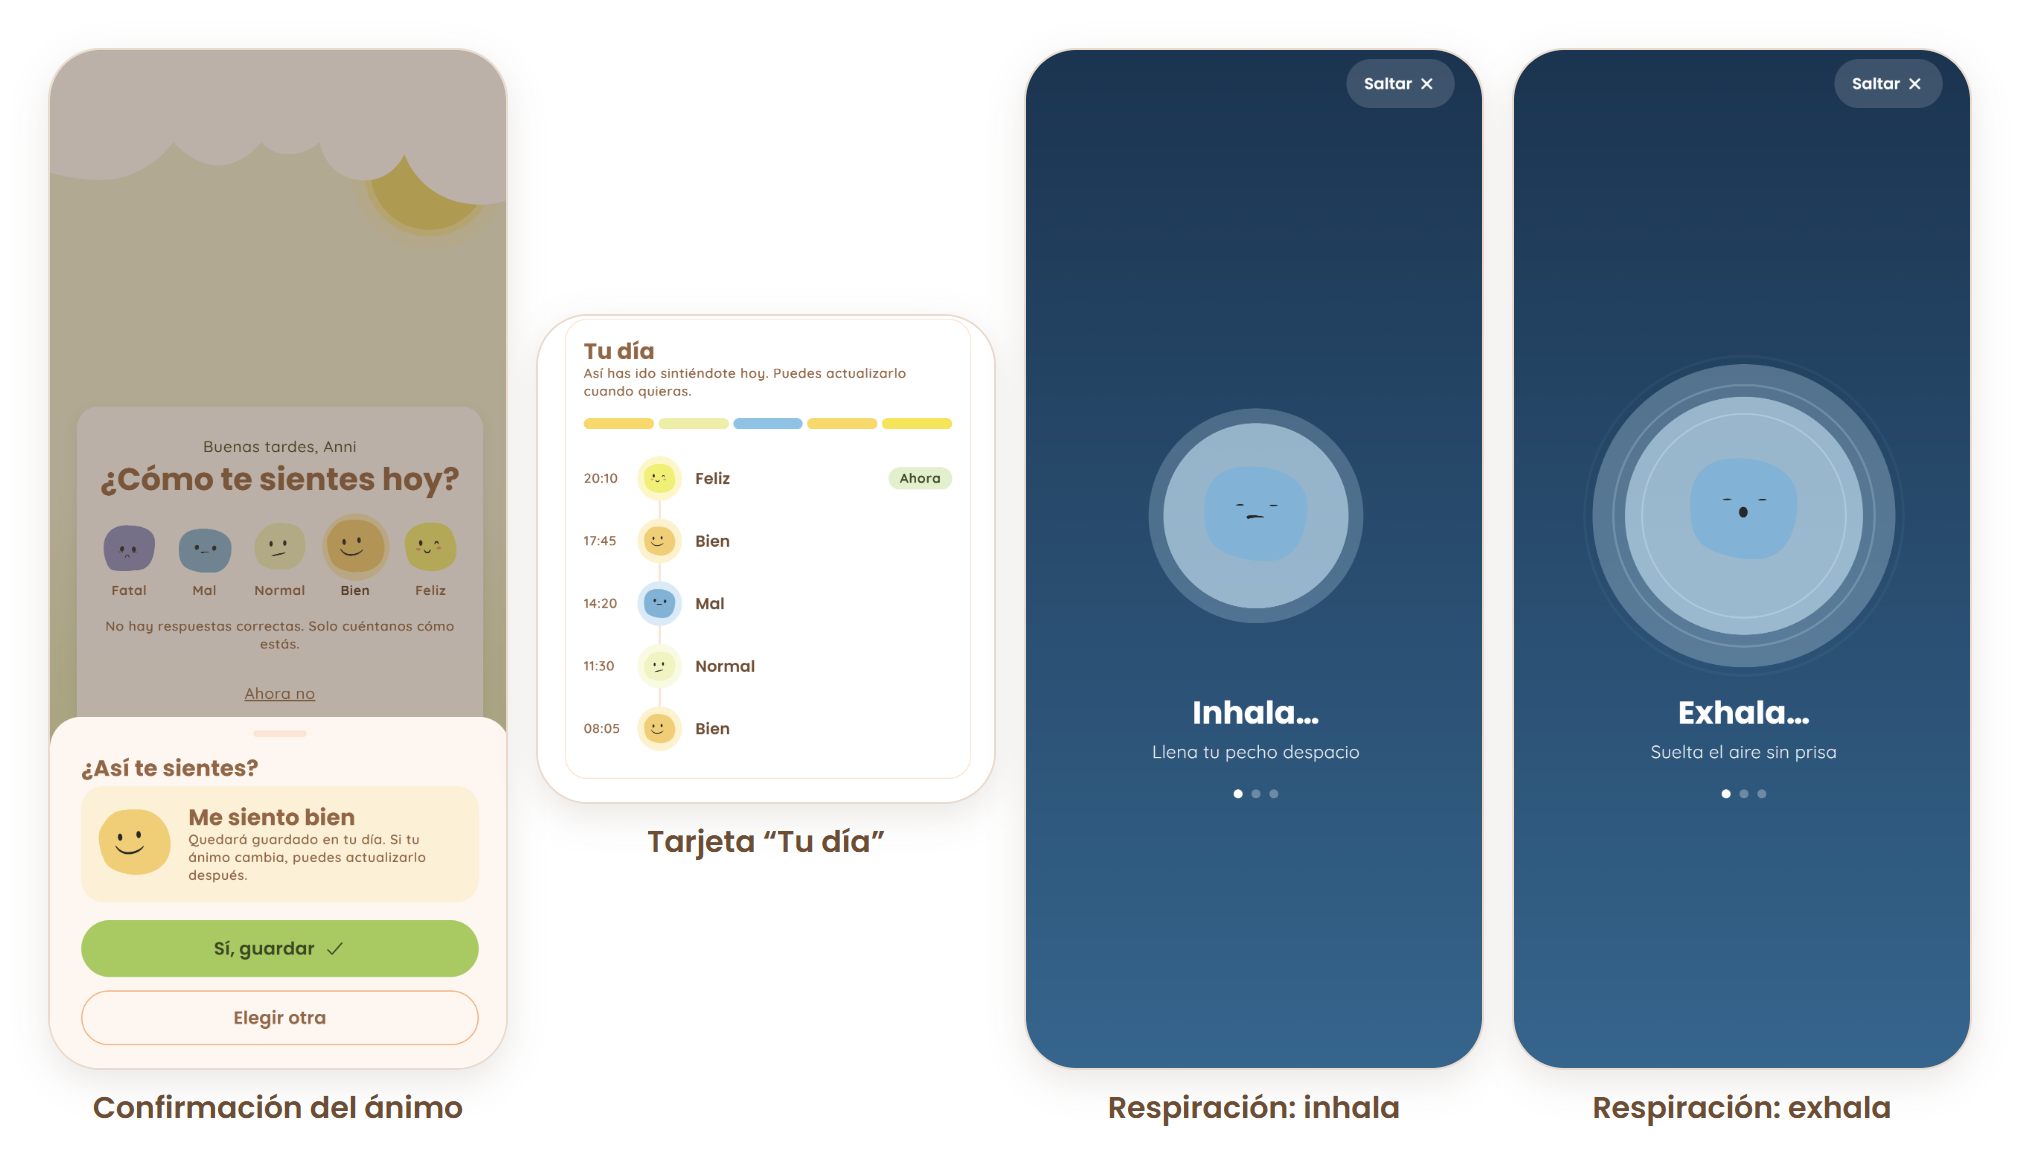
\includegraphics[width=\textwidth]{Images/methodology/prototype/mood.png}
  \vspace{4pt}
\end{figure}

\subsection{Tono del mensaje y reacciones}
Para compensar la falta de señales no verbales en el texto (Picard, 1997), cada mensaje puede llevar de manera opcional un \textbf{tono}: \textit{con cariño}, \textit{en broma}, \textit{para animarte}, \textit{con curiosidad}, \textit{con gratitud} o \textit{en serio}. La burbuja adopta un tinte suave del tono elegido, muestra una etiqueta con su ícono y, al llegar, entra con un gesto propio. Quien escribe tiende a sobreestimar cuánto se entiende su tono, y los lectores distinguen una broma de un mensaje serio apenas por encima del azar (Kruger et al., 2005); declarar el tono reduce los malentendidos con alguien a quien todavía no se conoce.

Asimismo, al mantener presionado un mensaje recibido aparecen cinco \textbf{reacciones}, representadas con las mismas caras de ánimo de la aplicación y con un sentido empático: \textit{Me alegra}, \textit{Me gusta}, \textit{Entiendo}, \textit{Lo siento} y \textit{Te abrazo}. Las señales gráficas cumplen en la comunicación escrita una función similar a la de los gestos (Derks et al., 2008). Las reacciones no descuentan del límite diario de mensajes, y para no sumar opciones visibles en cada mensaje (Ley de Hick; Yablonski, 2020) solo aparecen cuando el usuario las solicita.

La Figura \ref{fig:conversacion} muestra una conversación con mensajes con tono, reacciones y la coincidencia revelada en un día.

\begin{figure}[htbp]
  \centering
  \caption{Conversación con mensajes con tono, reacciones y coincidencias del día}
  \label{fig:conversacion}
  \vspace{4pt}
  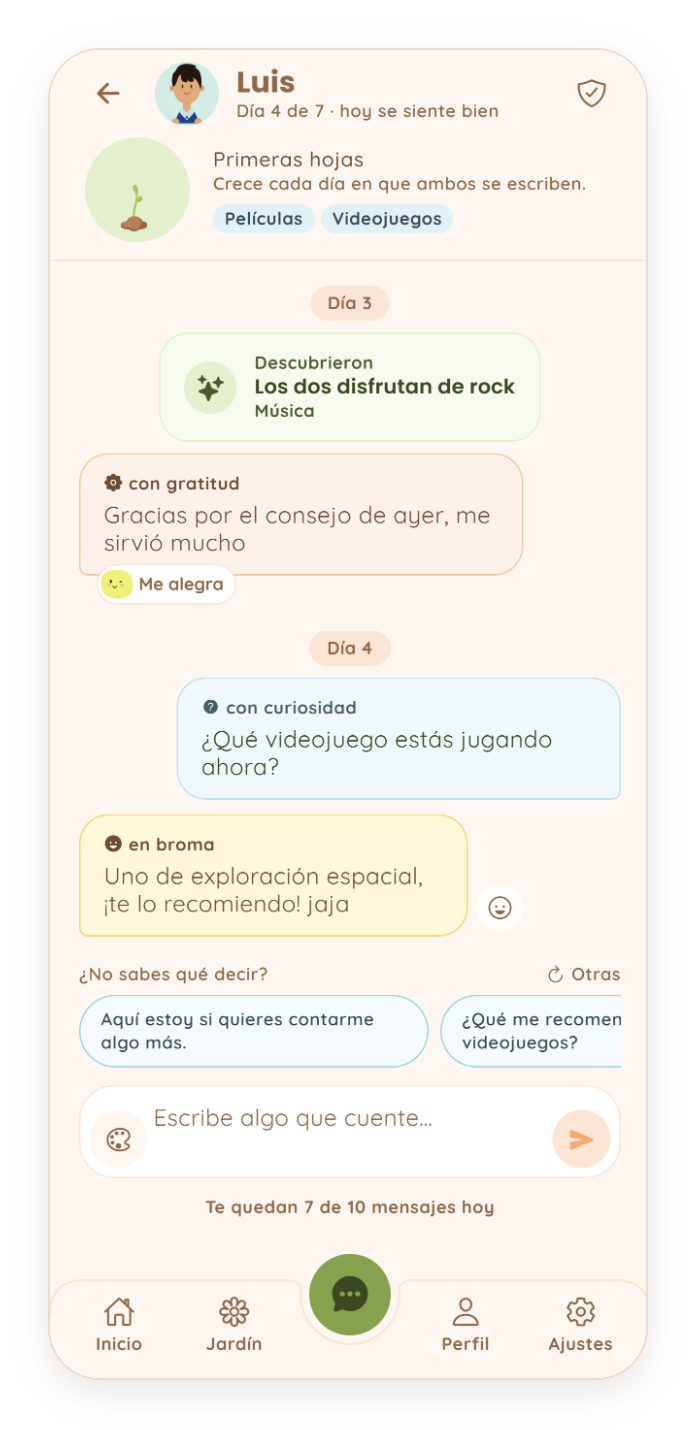
\includegraphics[width=0.4\textwidth]{Images/methodology/prototype/chat.png}
  \vspace{4pt}
\end{figure}

\subsection{Jardín}
El Jardín se diseñó como un lugar y no como una lista. Sobre un paisaje animado propio, las plantas de cada conversación quedan plantadas en las colinas, de izquierda a derecha y cada una un poco más arriba, como si el jardín subiera la colina; si no caben en la pantalla, el paisaje se desliza hacia la derecha. Sobre cada planta se muestra una etiqueta con el avatar, el nombre y la fecha de la otra persona. Al tocar una planta se abre una \textbf{postal de esa semana}, con lo que ambos descubrieron en común, las reacciones que se regalaron, el tono con que más se escribieron y el primer mensaje. Una metáfora espacial despierta más apego que un listado (nivel reflexivo del diseño emocional; Norman, 2004), y la postal convierte cada planta en un recuerdo con significado, sin cifras ni rachas y sin plantas que se marchiten, que generarían culpa o un uso compulsivo (Feng et al., 2026).

La Figura \ref{fig:jardin} muestra el Jardín y la postal que se abre al tocar una planta.

\begin{figure}[htbp]
  \centering
  \caption{Jardín y postal de una semana}
  \label{fig:jardin}
  \vspace{4pt}
  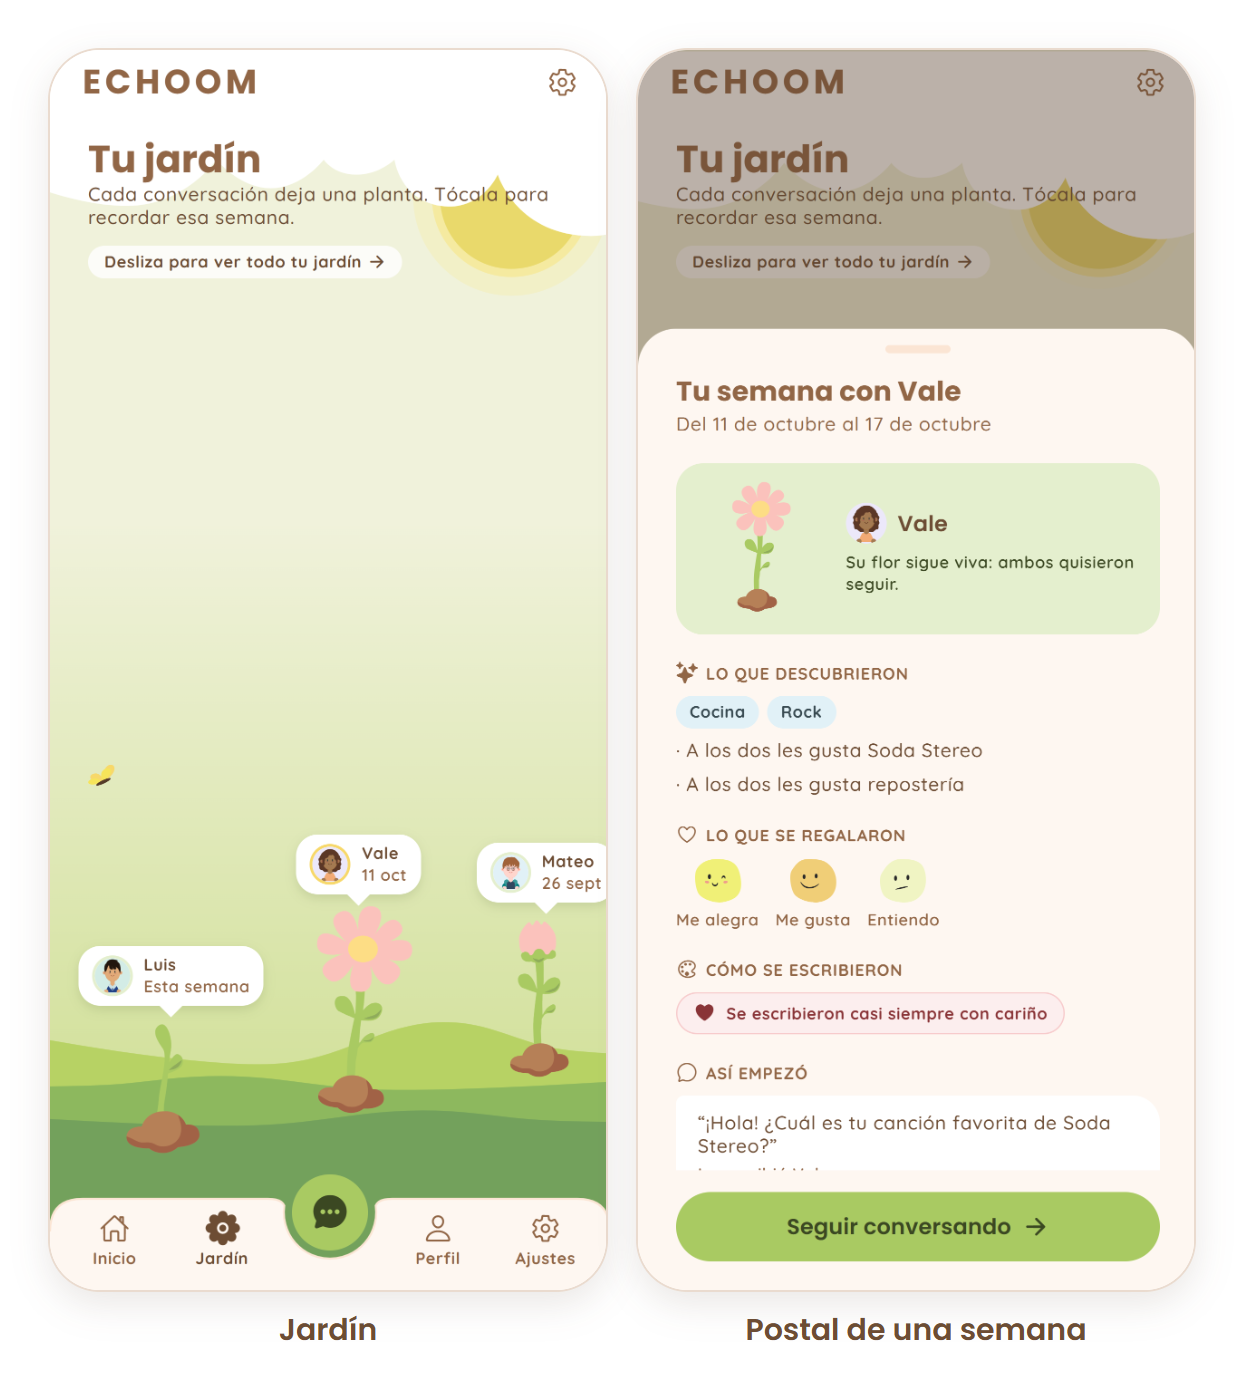
\includegraphics[width=0.7\textwidth]{Images/methodology/prototype/garden.png}
  \vspace{4pt}
\end{figure}

\subsection{Micro-interacciones}
Las micro-interacciones del prototipo se diseñaron siguiendo la definición de Saffer (2013), quien sostiene que su poder reside en la brevedad: no requieren un compromiso prolongado del usuario para generar un efecto significativo. Entre las implementadas en ECHOOM se encuentran:

\begin{itemize}
    \item La primera vez de cada día que se abre la conversación, una pantalla breve muestra la planta sobre un paisaje animado con el texto ``Día N de 7''. Si creció desde la última visita, se la ve crecer con destellos y el aviso ``¡Su planta creció!''; si no, recorre sus etapas y recuerda que ese día pueden hacerla crecer escribiéndose ambos. Esta retroalimentación inmediata ante un comportamiento recíproco se alinea con los hallazgos de Godard y Holtzman (2024) sobre el valor del uso activo y recíproco.
    \item Una animación de búsqueda con mensajes que cambian progresivamente, reduciendo la percepción de espera mientras el sistema localiza una posible pareja (Umbral de Doherty; Yablonski, 2020). Si el usuario sale de esa pantalla, la búsqueda continúa y la tarjeta de Inicio se actualiza sola hasta avisar ``¡Encontramos a alguien!''.
    \item Al registrar el ánimo, la cara elegida reacciona y la tarjeta se recoge en un resumen (``Hoy te sientes bien''), con la opción de actualizarlo, ofreciendo retroalimentación informativa inmediata (Shneiderman et al., 2016).
    \item Los botones, chips y pestañas se hunden levemente al tocarlos y regresan con un rebote suave, de modo que el toque se confirma con movimiento y no solo con color.
    \item La pantalla de cierre de cada semana fue diseñada con especial cuidado visual y de contenido, dado que, conforme a la Regla del Pico-Final, las personas juzgan una experiencia principalmente por su momento más intenso y por su cierre (Yablonski, 2020).
\end{itemize}

La Figura \ref{fig:crecimiento} muestra la pantalla diaria de la planta antes y después de crecer, y la pantalla de cierre cuando ambos deciden continuar.

\begin{figure}[htbp]
  \centering
  \caption{Crecimiento diario de la planta y cierre de la semana}
  \label{fig:crecimiento}
  \vspace{4pt}
  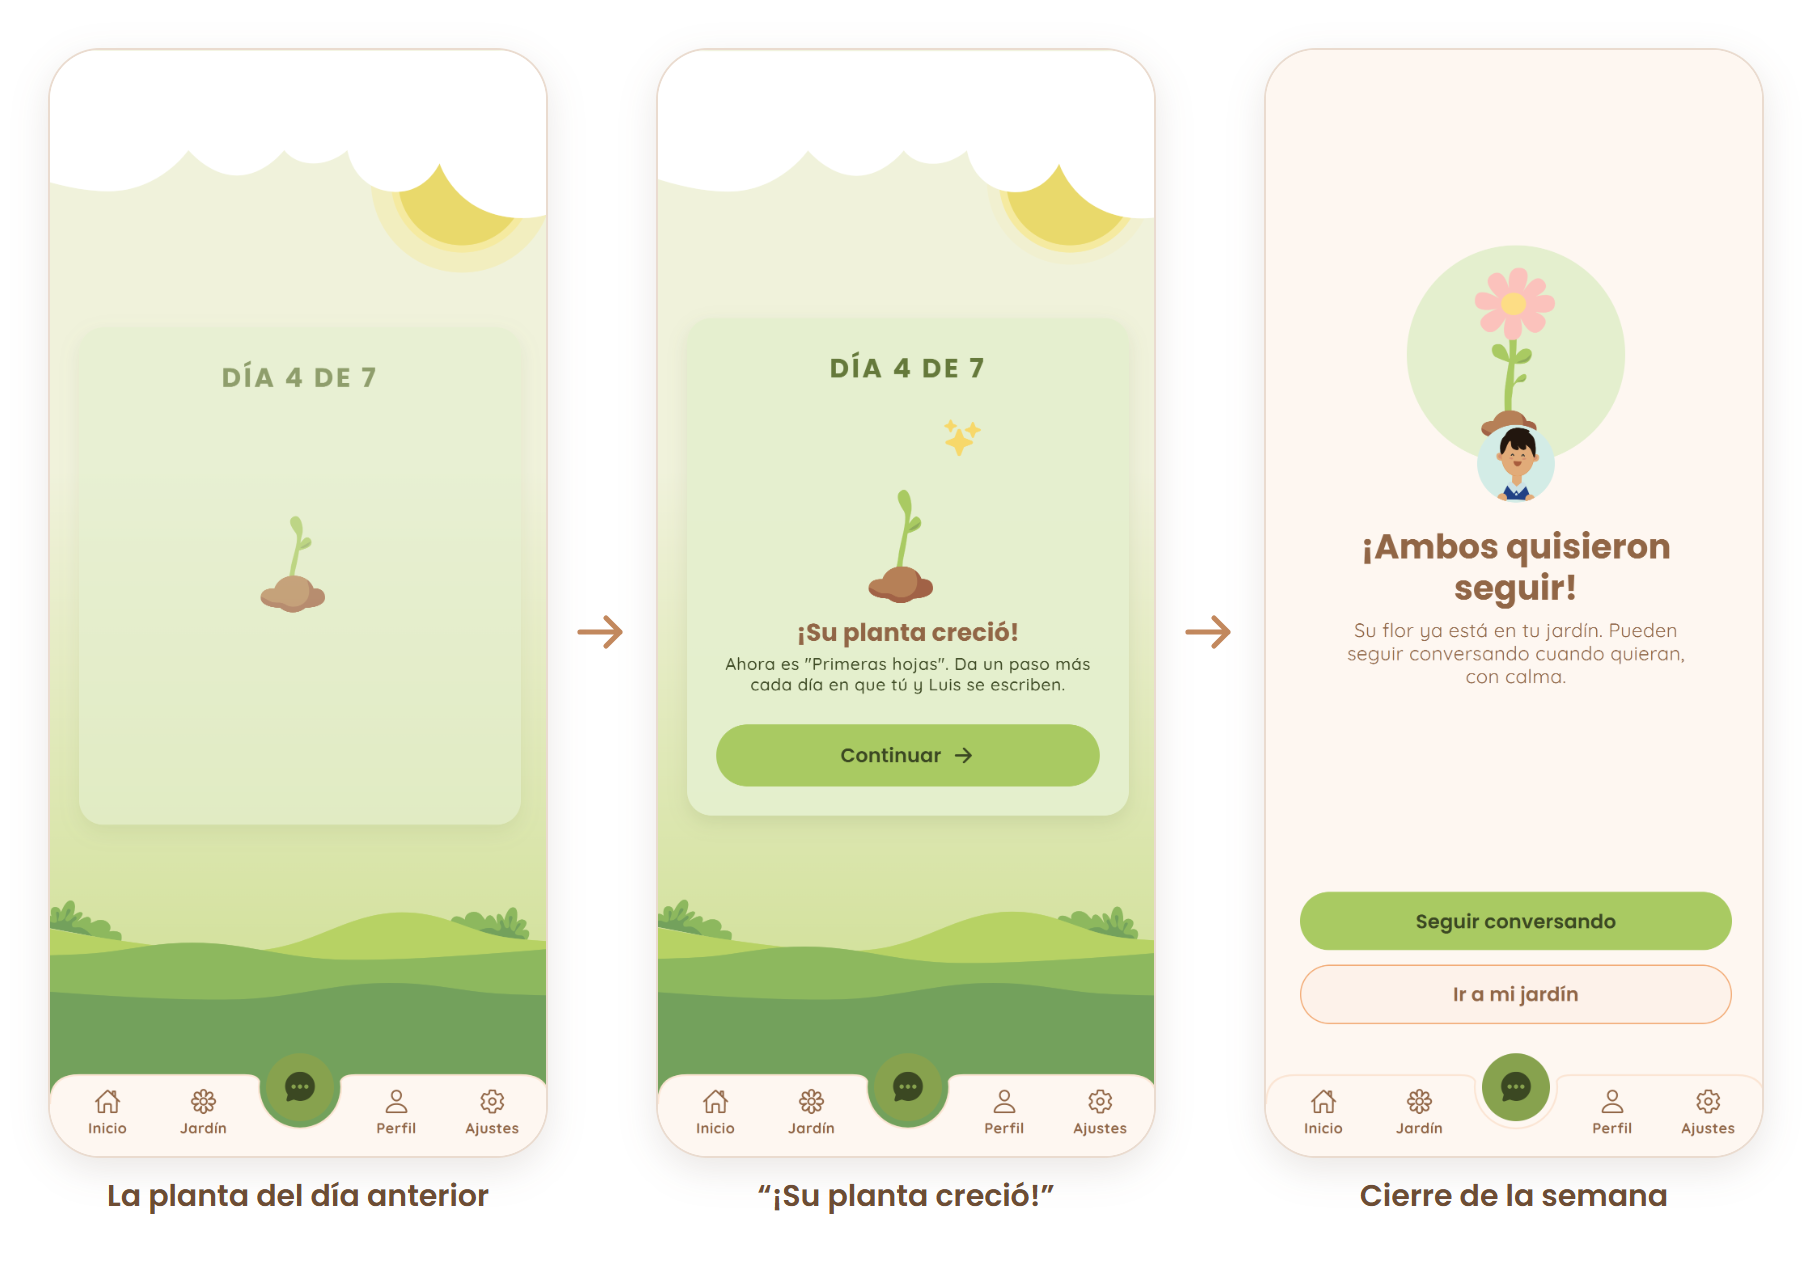
\includegraphics[width=0.9\textwidth]{Images/methodology/prototype/growth.png}
  \vspace{4pt}
\end{figure}

\subsection{Sonidos}
El prototipo incorpora sonidos propios, sintetizados para la aplicación, suaves y de menos de cuatro segundos, que se reproducen únicamente en momentos con significado: cada ánimo suena distinto al elegirlo, sin que ninguno suene a error; en la respiración guiada, un cuenco marca el inicio de la inhalación y otro el de la exhalación, de modo que el ejercicio pueda seguirse con los ojos cerrados; la planta suena al crecer y al florecer; al abrir el recuerdo de una planta en el Jardín suena una pequeña caja de música; y existen avisos al encontrar pareja, al enviar, al recibir un mensaje con la conversación abierta y al reaccionar. Los íconos auditivos (Gaver, 1986) y los \textit{earcons} (Blattner et al., 1989) refuerzan la retroalimentación sin ocupar la pantalla, y su uso escaso responde al principio de tecnología calmada (Weiser \& Brown, 1996). Los botones y las pestañas no suenan; los sonidos pueden desactivarse en Ajustes, respetan el modo silencio del teléfono, no interrumpen la música del usuario y nunca son el único canal de información, pues todo se muestra también en pantalla (W3C, 2023).

\subsection{Lenguaje del sistema}
Todos los mensajes generados por el sistema (avisos, confirmaciones, estados de espera) se redactaron en segunda persona, con un tono cálido y libre de culpa. Por ejemplo, al agotarse los mensajes diarios el sistema indica ``Ya compartiste tus mensajes de hoy. Mañana podrás escribir de nuevo'', en lugar de un aviso de error genérico; y la opción de abandonar una conversación se etiqueta como ``Cerrar aquí''. Esta decisión responde al enfoque afectivo de la IHC, que no solo busca que la interacción resulte placentera, sino también influir en las emociones y actitudes del usuario respecto al uso del sistema (Gupta, 2012, como se citó en Méndez et al., 2014), y a la recomendación de ofrecer instrucciones sencillas y constructivas cuando el usuario no puede completar una acción (Shneiderman et al., 2016).

\subsection{Diseño adaptable}
La interfaz se adapta a teléfonos pequeños, grandes y tablets. En la pantalla de Inicio, el contenido ocupa todo el ancho disponible y conserva el mismo orden en cualquier tamaño de pantalla, evitando el uso de columnas múltiples que fragmenten la atención del usuario, en coherencia con la Ley de Miller sobre la capacidad limitada de la memoria de trabajo (Yablonski, 2020).

\section{HACIA LA FASE TESTEAR}
Las decisiones de diseño descritas en este capítulo constituyen un conjunto de hipótesis que deberán validarse con usuarios reales durante la prueba piloto, desarrollada en el Capítulo 9. En particular, interesa conocer si la duración de siete días y el límite de diez mensajes diarios resultan adecuados, si las ideas para romper el hielo y las coincidencias reveladas cada día cumplen su función, si la representación del vínculo mediante una planta motiva la interacción sin generar presión, y si la moderación antes de enviar se percibe como cuidado y no como censura, en coherencia con el principio de poner los prototipos en manos de los usuarios para recopilar retroalimentación cualitativa y cuantitativa (Vargas Márquez et al., 2021).
